\documentclass{article}[a4paper, 12pt]
\usepackage{minted}
\usepackage{csquotes}
\usepackage{french}
\usepackage{hyperref}
\usepackage{stackengine}
\usepackage[top=2.54cm, bottom=2.54cm, left=2.54cm, right=2.54cm]{geometry}
\usepackage[T1]{fontenc}
\usepackage{graphicx}
\usepackage[table]{xcolor}
\usepackage{copyrightbox}
\usepackage{multirow}%tableaux
\usepackage{listings} %cahier des besoins
\usepackage{bbding}
\usepackage{pifont}
\usepackage{wasysym}
\usepackage{amssymb}
\usepackage{enotez}

\def\FAIT{\textcolor[HTML]{4E944F}{\textbf{\ding{52}}}}
\def\NOP{\textcolor[HTML]{E83A14}{\textbf{\ding{55}}}}

\newcommand{\quotes}[1]{``#1''}

\lstset{
language=C,
extendedchars=true,
basicstyle=\tt,
%numbers=left, numberstyle=\tiny, stepnumber=2, numbersep=5pt,
lineskip=-1pt
}

\bibliographystyle{alpha} %format des citations

\title{\LARGE \textbf{Mémoire Projet de Programmation  } \\ \Large \textbf{Jeu de statégie : Desert Fox}}
\author{Kristo Dhima, Garion Goubard, Sylvain Lascostes, \\Romain Réau, Vincent Samson et Alexandros Stergiou }
\date{Année universitaire 2021-2022}

\begin{document}

\maketitle
\begin{center}
    \center
    
\includegraphics[scale=0.2]{data/Universite_Bordeaux_RVB-10.jpg}

\end{center}

\newpage

{\hypersetup{hidelinks} \tableofcontents} %table des matière


\newpage

\section{Description du projet}

Le but de ce projet est de réaliser le moteur du jeu de guerre \emph{Desert Fox}.
Le moteur du jeu contiendra une architecture qui puisse se déployer à travers Internet ou en local.
Les scénarios seront mis de côté afin de réaliser au mieux le moteur.\\

Deux joueurs vont devoir s'affronter sur une carte composée d'une grille d'hexagones.
Le but du joueur de l'Axe est de sécuriser la Libye et l'Égypte en s'emparant d'Alexandrie, tandis que, le joueur Allié (Commonwealth et autres) protège Alexandrie et doit contenir les forces du joueur opposé.\\
Le joueur Allié a 38 tours pour protéger Alexandrie.

Chaque tour possède plusieurs étapes :
\begin{itemize}
    \item Préparation
    \item Une suite de phases (20) d'actions où les joueurs bougent leurs unités et les engagent au combat.
          Cette partie est divisée en 4 phases distinctes, où le premier joueur alterne entre Allie et Axe à chaque fois :
          \begin{itemize}
              \item Mouvement du premier joueur.
              \item Réaction du second joueur.
              \item Combat du premier joueur.
          \end{itemize}
    \item Phase de fin de jeu, c'est-à-dire vérification des approvisionnements, de la victoire et de la fin de la partie.
\end{itemize}


La partie est hébergée sur un serveur afin de centraliser les données de la partie et simplifier les échanges client $\leftrightarrow$ serveur.

\section{Analyse de l'existant}

Divers projets open-source proposent des moteurs de jeu \emph{wargame}. Cependant, la plupart de ces projets ne sont pas maintenus depuis plusieurs années où ne sont pas adaptées pour nos besoins.
Le nombre de règles et d'extensions est énorme et leur adaptation à un moteur de jeu déjà existant est complexe.
De ce fait, nous avons décidé de créer un moteur de jeu nous même qui convient parfaitement au jeu.
\begin{figure}[H]
    \centering
    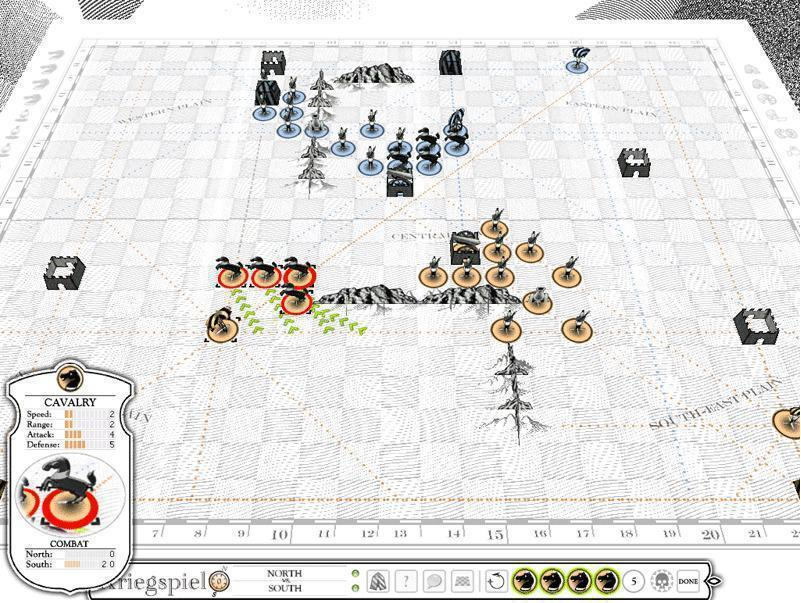
\includegraphics[scale=0.5]{data/kriegspiel.jpeg}\\
    Source : \endnote{\url{https://download.tuxfamily.org/sdtraces/BottinHTML/Bottin_K-O_files/38e33e3e441a297d6fc55b27dd6a98d3.jpeg}}
    \caption{Jeu \textit{Kriegspiel} : Plateau du jeu}
\end{figure}


Par exemple, Nous avons trouvé un jeu similaire à notre projet : \textit{Kriegspiel}, un des plus anciens jeux de guerre, datant du XIXe siècle, initialement créé par des généraux Prussiens pour former leurs officiers, adapté aussi dans des versions plus modernes.
C'est un jeu de pions complexe   \cite{livermore1879american}
\begin{figure}[H]
    \centering
    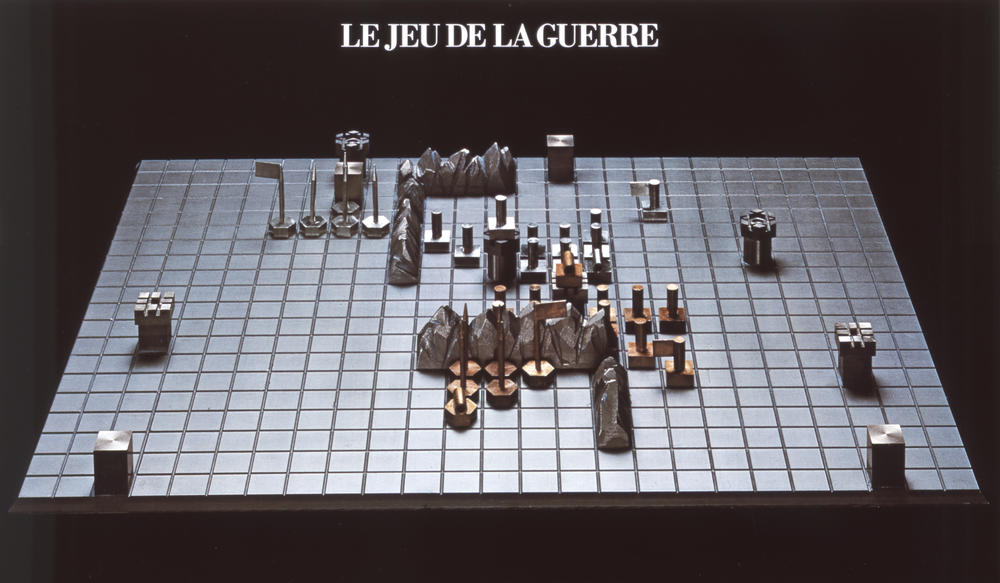
\includegraphics[scale=1.0]{data/Cavalry_at_dusk.jpg}\\

    Source : \endnote{\url{https://www.telerama.fr/sites/tr_master/files/styles/simplecrop1000/public/illustrations/thumbnails/jeudelaguerre_2.jpg?itok=yKwqIeaD}}
    \caption{\textit{Le Jeu de la guerre (War Game)} : Plateau du jeu}.

\end{figure}

Le Jeu de la Guerre \cite{frwiki:189457170} est un essai stratégique de Guy Debord et Alice Becker-Ho édité en 1987.
C'est un jeu qui se joue sur un plateau de 25x20. Contrairement à Desert Fox le plateau contient des cases carrées. La ressemblance avec Desert Fox est la formation d'unité (infanterie, cavalerie, artillerie).
Le but du jeu, est de vaincre l'adversaire, soit en détruisant son arsenal ou toutes ses unités. À chaque tour, un joueur peut déplacer cinq unités.


\begin{figure}[H]
    \centering
    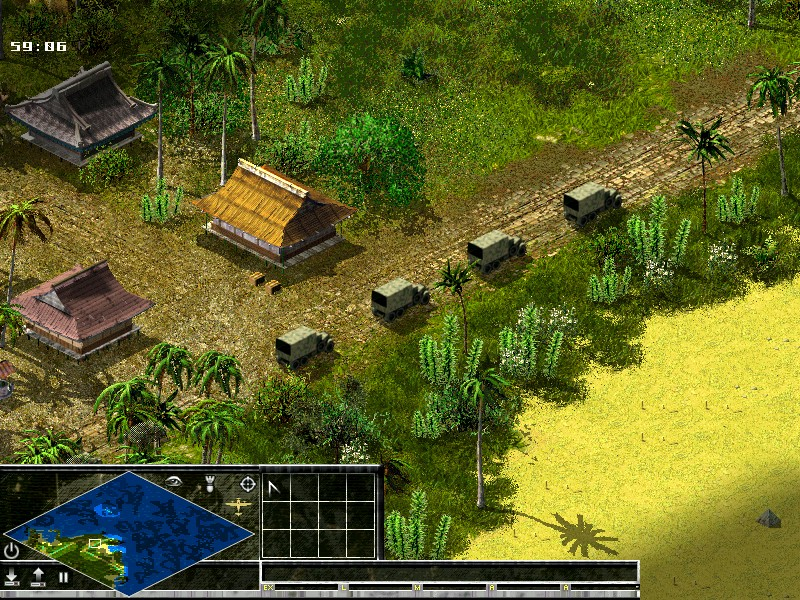
\includegraphics[scale=0.3]{data/sudden_strike_2.jpg}\\
    Source : \endnote{\url{https://cdn.cloudflare.steamstatic.com/steam/apps/612520/ss_e593c9966bc58b7326287db455776b2291718f76.600x338.jpg?t=1644312432}}
    \caption{\textit{Sudden Strike 2 Gold} : Le jeu propose cinq campagnes, une par faction, composée chacune d’une dizaine de missions : l'URSS, le Japon, l'Allemagne, États-Unis et Royaumes-Unis.}
\end{figure}

Sudden Strike 2 est un jeux-vidéo sortie en 2002. Il s'agit du deuxième volet de la série Sudden Strike. C'est un jeu datant de la seconde guerre mondiale.
Le joueur peut commander les force de l’Allemagne, de l’URSS, du Japon, des États-Unis ou du Royaume-Uni.
Le joueur commence avec un nombre prédéfini d'unités. Ce jeu propose différents scénarios. Plus de 50 unités sont proposées dont : infanterie, char d'assaut, artillerie et aviation.
Il est possible de transporter des troupes, des véhicules et ravitaillements par le train, de mettre en place des ponts aériens ou organiser des opérations de parachutage.


\begin{figure}[H]
    \centering
    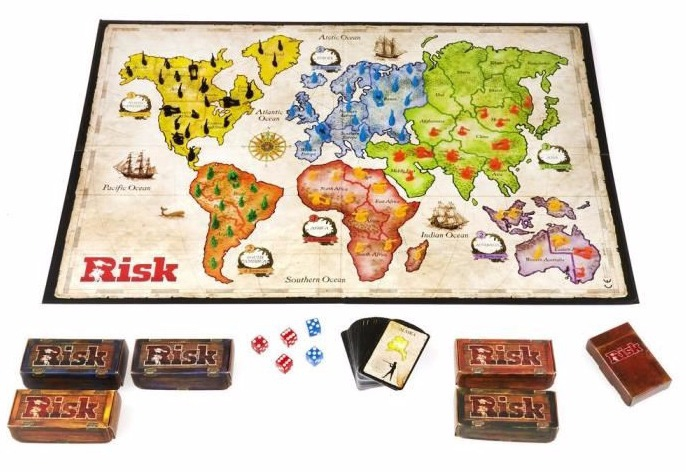
\includegraphics[scale=0.4]{data/risk.jpg}\\
    Source \endnote{\url{https://www.espritjeu.com/upload/image/risk-nouvelle-edition-p-image-60508-grande.jpg}}
    \caption{\textit{Risk nouvelle expédition} : Jeu société.}
\end{figure}
Risk est un jeu de société de guerre. Édité en 1957. Il est possible de jouer de 2 à 6 joueurs. Ce jeu peut durer jusqu'à 2 heures. À la différence des autres jeux, ce jeu se passe dans le monde entier. Le plateau représente la Terre.
Après la distribution des cartes, tous les joueurs posent un fantassin sur chacun de ces pays, puis le maître du jeu choisi une mission. Les joueurs doivent deviner la mission des adversaires.
Les joueurs peuvent bluffer.
Le but du jeu est d'allouer des armées dans les territoires contrôlés puis attaquer les zones voisines. Un participant est éliminé s’il ne lui reste plus de territoires.


\begin{figure}[H]
    \centering
    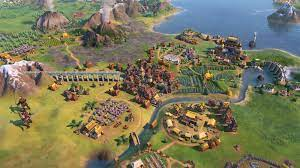
\includegraphics[scale=0.8]{data/civilization.jpeg}\\
    Source \endnote{\url{https://www.gamecash.fr/thumbnail-650/civilization-6-2-e146117.jpg}}
    \caption{\textit{civilization VI} : jeu vidéo.}
\end{figure}
Civilization VI est un jeu vidéo de stratégie. Il s'agit du sixième opus.
Le principe du jeu est de développer sa civilisation et de conquérir les autres, pour cela il existe plusieurs moyens :
\begin{itemize}
    \item Militaire : lorsqu'une civilisation a conquis toutes les capitales étrangères.
    \item Scientifique : lorsque que la première civilisation réussit à développer une colonie sur Mars.
    \item Culturelle : lorsqu'une civilisation accueille plus de touristes étrangers que les autres civilisations.
    \item Religieuse : lorsqu'une civilisation a réussi à convertir au moins 50\% de tous les citoyens de toutes les autres villes.
    \item Diplomatique : lorsque qu'une civilisation obtient un certain nombre de point diplomatique.
    \item Score : la civilisation qui a le plus de points au bout de 1500 tours.
\end{itemize}
Les possibilités sont multiples et chaque joueur peut choisir une stratégie pour l'emporter.




\newpage


\section{Descriptions des besoins}

\subsection{Besoins Fonctionnels}
\subsubsection{Plateau de Jeu}

\begin{center}
    \centering
    \begin{tabular}[h]{|m{14cm}|m{2cm}|}
        \hline
        \rowcolor[HTML]{FFA8A8}
        \multicolumn{2}{|c|}{\textbf{Priorité 3/3}}                                                                                                                  \\
        \hline
        Besoins                                                                                                                                         & Avancement \\
        \hline
        • Les hexagones numérotés, chacun représentant une distance définie, par défaut : 16 kilomètres                                                 & \FAIT      \\
        • Définir les joueurs et leurs spécificités. Par exemple les nationalités possibles, le joueur qui joue le premier et celui qui a l’initiative. & \FAIT      \\
        • Pouvoir poser des unités sur la carte et à retenir celles qui ne sont pas présentes dans celles-ci                                            & \FAIT      \\
        • Pouvoir poser plusieurs unités sur un hexagone                                                                                                & \FAIT      \\
        • Définir une séquence de tour :
        \begin{itemize}
            \item Pouvoir alterner entre les joueurs
            \item Respecter l’ordre strict d’un tour
        \end{itemize}
                                                                                                                                                        & \FAIT      \\
        • Afficher un terminal qui permettra aux joueurs de donner des commandes d'attaque ou mouvement                                                 & \FAIT      \\
        • Être capable de faire des lancés de dés et d’appliquer des modificateurs. La majeure partie du jeu se base sur les dés                        & \FAIT      \\
        • Pouvoir déterminer quel joueur a l’initiative                                                                                                 & \NOP       \\
        \hline
    \end{tabular}
\end{center}

\begin{center}
    \centering
    \begin{tabular}[h]{|m{14cm}|m{2cm}|}
        \hline
        \rowcolor[HTML]{FFB72B}
        \multicolumn{2}{|c|}{\textbf{Priorité 2/3}}                                                                                                                                           \\
        \hline
        Besoins                                                                                                                                                                  & Avancement \\
        \hline
        • Différencier plusieurs types de terrain, les montages, les mers de sable et les crêtes par exemple                                                                     & \FAIT      \\
        • Créer une base pour les cartes d’évènements. Celles-ci étant très différentes, l’implémentation sera limitée aux évènements génériques (non spécifiques aux scénarios) & \NOP       \\
        • Pouvoir charger la carte du jeu à partir d’un fichier \textsc{txt} ou \textsc{json} et pouvoir la sauvegarder aux mêmes formats                                        & \FAIT      \\
        \hline
    \end{tabular}
\end{center}

\begin{center}
    \centering
    \begin{tabular}[h]{|m{14cm}|m{2cm}|}
        \hline
        \rowcolor[HTML]{C0D8C0}
        \multicolumn{2}{|c|}{\textbf{Priorité 1/3}}                                                                                  \\
        \hline
        Besoins                                                                                                         & Avancement \\
        \hline
        • Ajouter les différents types d’indicateurs afin d’illustrer les villages, les villes et les oasis par exemple & \FAIT      \\
        \hline
    \end{tabular}
\end{center}

\subsubsection{API}

\begin{center}
    \centering
    \begin{tabular}[h]{|m{14cm}|m{2cm}|}
        \hline
        \rowcolor[HTML]{FFA8A8}
        \multicolumn{2}{|c|}{\textbf{Priorité 3/3}}                                                                                               \\
        \hline
        Besoins                                                                                                                      & Avancement \\
        \hline
        • Pouvoir échanger des informations basiques entre serveur et client                                                         & \FAIT      \\
        • Pouvoir convertir un état de la carte du jeu en format utilisable par le client pour pouvoir ensuite afficher le plateau   & \FAIT      \\
        • Envoyer un coup joue dans un format utile pour le serveur, pour pouvoir faire des éventuelles modifications sur le plateau & \FAIT      \\
        • Vérification des coups :
        \begin{itemize}
            \item Envoyer le coup joue au serveur
            \item Vérifier que le coup est valide
            \item Retourner une réponse positive ou négative. Si le coup est bon alors envoyer le nouvel état de la carte du jeu au client
        \end{itemize}
                                                                                                                                     & \FAIT      \\
        \hline
    \end{tabular}
\end{center}

\subsubsection{Unités}

\begin{center}
    \centering
    \begin{tabular}[h]{|m{14cm}|m{2cm}|}
        \hline
        \rowcolor[HTML]{FFA8A8}
        \multicolumn{2}{|c|}{\textbf{Priorité 3/3}}                                                                                                                            \\
        \hline
        Besoins                                                                                                                                                   & Avancement \\
        \hline
        • Définir l'unité comme interface, qui aura une morale, peut être perturbée (disrupted) et qui peut prendre des actions basiques comme attaquer et bouger & \FAIT      \\
        • Implémenter le système similaire à des points de vie (voir partie \textit{Depletion} des règles)                                                        & \FAIT      \\
        • Séparer les unités en catégories différentes : motorisées, à pied, mécanisées, cavalerie...                                                             & \FAIT      \\
        • Mettre en place les situations ou l'unité devient perturbée :                                                                                                        \\
        \hspace*{10mm} \- Résultat d'un combat                                                                                                                    & \FAIT      \\
        \hspace*{10mm} \- Trop de troupes sur un hexagone                                                                                                         & \FAIT      \\
        \hspace*{10mm} \- Fin d'un mouvement de nuit                                                                                                              & \NOP       \\
        \hspace*{10mm} \- Au début d'une phase de mouvement, si l'unité n'a pas accès à l'approvisionnement                                                       & \FAIT      \\
        \hline
    \end{tabular}
\end{center}

\begin{center}
    \centering
    \begin{tabular}[h]{|m{14cm}|m{2cm}|}
        \hline
        \rowcolor[HTML]{FFB72B}
        \multicolumn{2}{|c|}{\textbf{Priorité 2/3}}                                                \\
        \hline
        Besoins                                                                       & Avancement \\
        \hline
        • Permettre aux unités éligibles de s'entraîner et de faire des améliorations & \NOP       \\
        \hline
    \end{tabular}
\end{center}

% \subsubsection{Organisation de l'armée}


\subsubsection{Mouvement}

\begin{center}
    \centering
    \begin{tabular}[h]{|m{14cm}|m{2cm}|}
        \hline
        \rowcolor[HTML]{FFA8A8}
        \multicolumn{2}{|c|}{\textbf{Priorité 3/3}}                                                                                                       \\
        \hline
        Besoins                                                                                                                              & Avancement \\
        \hline
        • Déplacement case par case et enlever les points de mouvement correspondants de l'unité. Ceci pour limiter la capacité de mouvement & \FAIT      \\
        \hline
    \end{tabular}
\end{center}

\begin{center}
    \centering
    \begin{tabular}[h]{|m{14cm}|m{2cm}|}
        \hline
        \rowcolor[HTML]{C0D8C0}
        \multicolumn{2}{|c|}{\textbf{Priorité 1/3}}                                                                            \\
        \hline
        Besoins                                                                                                   & Avancement \\
        \hline
        • Le joueur Allié peut accélérer le mouvement de ses unités en utilisant le rail et le transport maritime & \NOP       \\
        • Avoir les types de mouvement speciaux: 
        \begin{itemize}
            \item Mouvement sur une route pour avancer plus vite
            \item Mouvement forcée pour bouger plus vite mais recevoir des effets négatifs à la fin du mouvement
        \end{itemize} & \NOP       \\
    \end{tabular}
\end{center}

\begin{center}
    \centering
    \begin{tabular}[h]{|m{14cm}|m{2cm}|}
        \hline
        \rowcolor[HTML]{FFB72B}
        \multicolumn{2}{|c|}{\textbf{Priorité 2/3}}                                                                                                                                                                                                                                                                        \\
        \hline
        Besoins                                                                                                                                                                                                                                                                                               & Avancement \\
        \hline
        • Déplacement d'un point A à un point B, en parcourant le plus cours chemin. On utilisera l'algorithme {\tt Dijkstra} pour satisfaire la condition                                                                                                                                                    & \FAIT      \\
        • Appliquer un bonus de mouvement dépendant du terrain d'un hexagone. Il est plus facile de se déplacer sur une plaine plutôt que sur une montagne                                                                                                                                                    & \FAIT      \\
        • Permettre aux unités qui doivent se replier de bouger de 1-3 hexagones. Ce mouvement ne coûte pas de points de mouvement                                                                                                                                                                            & \FAIT      \\
        • Ajouter la mécanique du {\tt overrun} (fuite). Les unités capables de le faire peuvent pendant leur phase de mouvement attaquer des unités. Les défenseurs alors peuvent utiliser leurs phases de réaction pour bouger un certain nombre d'hexagones. La distance est définie par l'unité concernée & \NOP       \\
        \hline
    \end{tabular}
\end{center}

\begin{center}
    \centering
    \begin{tabular}[h]{|m{14cm}|m{2cm}|}
        \hline
        \rowcolor[HTML]{C0D8C0}
        \multicolumn{2}{|c|}{\textbf{Priorité 1/3}} \\
        \hline
        Besoins             & Avancement            \\
        \hline
        • Mouvement la nuit & \NOP                  \\
        \hline
    \end{tabular}
\end{center}

\subsubsection{Combat}

\begin{center}
    \centering
    \begin{tabular}[h]{|m{14cm}|m{2cm}|}
        \hline
        \rowcolor[HTML]{FFA8A8}
        \multicolumn{2}{|c|}{\textbf{Priorité 3/3}}                                                                                                                                                                                                                                                                                                                                        \\
        \hline
        Besoins                                                                                                                                                                                                                                                                                                                                                               & Avancement \\
        \hline
        • Pouvoir définir les unités participant à un combat                                                                                                                                                                                                                                                                                                                  & \FAIT      \\
        • Pouvoir déterminer la puissance de combat de l'armée composée de ces unités                                                                                                                                                                                                                                                                                         & \FAIT      \\
        • Définir les règles du combat, par exemple le fait que seules les unités/armées adjacentes peuvent entrer en combat, par la volonté de l'attaquant                                                                                                                                                                                                                   & \FAIT      \\
        • Pouvoir simuler le combat et donner les résultats :
        \hspace*{10mm} \- Déterminer les dégâts causés par une unité en divisant le nombre d'attaquants par le nombre de défenseurs de l'ennemie pour obtenir un ratio.                                                                                                                                                                                                       & \FAIT      \\
        \hspace*{10mm} \- Séparer les défenseurs en groupe de morale. Les unités avec le même morale se retrouvent dans le même groupe. Les résultats seront dans l'ordre descendant de morale. Par exemple si on a deux groupes de morale (de 1 et 2), alors les résultats du combat seront d'abord appliqués dans le groupe avec une morale de 2, puis a celui de morale 1. & \FAIT      \\
        \hspace*{10mm} \- Appliquer des éventuelles règles spéciales.                                                                                                                                                                                                                                                                                                         & \NOP       \\
        \hspace*{10mm} \- Si un hexagone contient que des unités de support, alors lancer un dé si l'attaquant le souhaite, pour tenter de capturer les unités.\newline Un résultat de 1-3 est un succès et un résultat de 4-6 veut dire que les unités de support sont détruites.                                                                                            & \FAIT      \\
        \hspace*{10mm} \- Amasser les dégâts et puis causer des dégâts aux unités adverses.\newline Les dégâts sont distribués parmi toutes les unités d'un groupe de morale.                                                                                                                                                                                                 & \FAIT      \\
        \hspace*{10mm} \- Enlever du plateau les unités détruites, et les ajouter dans la liste d'unités détruites du joueur concernée.                                                                                                                                                                                                                                       & \FAIT      \\
        \hspace*{10mm} \- Lancer un dé pour faire le test de morale des unités qui reste. Si le test échoue, alors l'unité est {\tt disrupted}.                                                                                                                                                                                                                                 & \FAIT      \\                                                                                                                                                 & ?          \\
        • Pouvoir simuler la retraite d'une armée si les spécifications le permettent, par exemple le terrain et la condition de l'armée est convenable, et si l'utilisateur le souhaite                                                                                                                                                                                      & \FAIT      \\
        \hline
    \end{tabular}
\end{center}

\begin{center}
    \centering
    \begin{tabular}[h]{|m{14cm}|m{2cm}|}
        \hline
        \rowcolor[HTML]{C0D8C0}
        \multicolumn{2}{|c|}{\textbf{Priorité 1/3}}                                                                         \\
        \hline
        Besoins                                                                                                & Avancement \\
        \hline
        • Si un {\tt Hex} contient plusieurs terrains, le défenseur doit pouvoir en choisir un pour sa défense & \NOP       \\
        \hline
    \end{tabular}
\end{center}

\subsubsection{Opérations Aériennes et Navales}

\begin{center}
    \centering
    \begin{tabular}[h]{|m{14cm}|m{2cm}|}
        \hline
        \rowcolor[HTML]{C0D8C0}
        \multicolumn{2}{|c|}{\textbf{Priorité 1/3}}                                                                                                                                       \\
        \hline
        Besoins                                                                                                                                                              & Avancement \\
        \hline
        • Pouvoir déterminer les différentes unités aériennes et navales ainsi que leurs spécificités                                                                        & \NOP      \\
        • Pouvoir déterminer les différentes cibles, par exemple des bases militaires ou les rivages(pour les opérations navales surtout), qu'ils peuvent cibler et attaquer & \NOP      \\
        • En ce qui concerne les opérations navales, ils peuvent effectuer des expéditions transportant des munitions ainsi que des unités/machines de guerre                & \NOP      \\
        \hline
    \end{tabular}
\end{center}

\subsubsection{Affichage}

\begin{center}
    \centering
    \begin{tabular}[h]{|m{14cm}|m{2cm}|}
        \hline
        \rowcolor[HTML]{FFA8A8}
        \multicolumn{2}{|c|}{\textbf{Priorité 3/3}}                                                                                                   \\
        \hline
        Besoins                                                                                                                          & Avancement \\
        \hline
        • Afficher le joueur dont c'est le tour                                                                                          & \FAIT      \\
        • Déterminer et afficher les informations de fin de partie et du vainqueur                                                       & \FAIT      \\
        • Afficher les différents marqueurs sur l'état de chaque composante du jeu, par exemple hors d'approvisionnement pour les unités & \FAIT      \\
        • Afficher le résultat et les informations à la fin du combat                                                                    & \FAIT      \\
        • Affiche un message d'erreur ou de refus quand une requête ou commande invalide est entrée.                                     & \FAIT      \\
        \hline
    \end{tabular}
\end{center}

\subsubsection{Réseaux}

\begin{center}
    \centering
    \begin{tabular}[h]{|m{14cm}|m{2cm}|}
        \hline
        \rowcolor[HTML]{FFA8A8}
        \multicolumn{2}{|c|}{\textbf{Priorité 3/3}}                                                                                                       \\
        \hline
        Besoins                                                                                                                              & Avancement \\
        \hline
        • Le jeu sera autour d'une architecture client-serveur qui puisse se déployer à travers Internet (pas seulement sur un réseau local) & \FAIT      \\
        \hline
    \end{tabular}
\end{center}

\subsection{Besoins Non-Fonctionnels}

\subsubsection{Affichage}
\begin{itemize}
    \item Le système doit être robuste aux erreurs de saisie et aux erreurs du serveur.
    \item Mettre en place une interface graphique affichant le plateau du jeu, les unités.
    \item Afficher un message d'attente au joueur qui ne joue pas.
\end{itemize}

\subsubsection{Système}
\begin{itemize}
    \item Le temps d'attente entre un coup proposé et sa validité évalué devront être de l'ordre de la seconde.
    \item Un chat sera créé pour communiquer avec l'adversaire.
\end{itemize}

\section{Scénario}

Les joueurs devront se connecter sur un serveur afin d'accéder à la partie. Le serveur hébergera la partie en traitant les mécanismes de la partie en arrière-plan. Les utilisateurs recevront une interface graphique en provenance du serveur et communiqueront avec cette interface pour jouer dans la partie.
Le serveur avertira l'utilisateur lors d'une mauvaise utilisation de l'interface et des requêtes parasites pour le serveur.




La carte s'affiche quand les deux joueurs sont connectés. Ici le joueur 1 peut commencer à jouer.
Nous pouvons voir en haut de la page une barre qui affiche le tour actuel sur 48, la phase actuelle et le nombre d'unités restantes.

\begin{figure}[H]
    \centering
    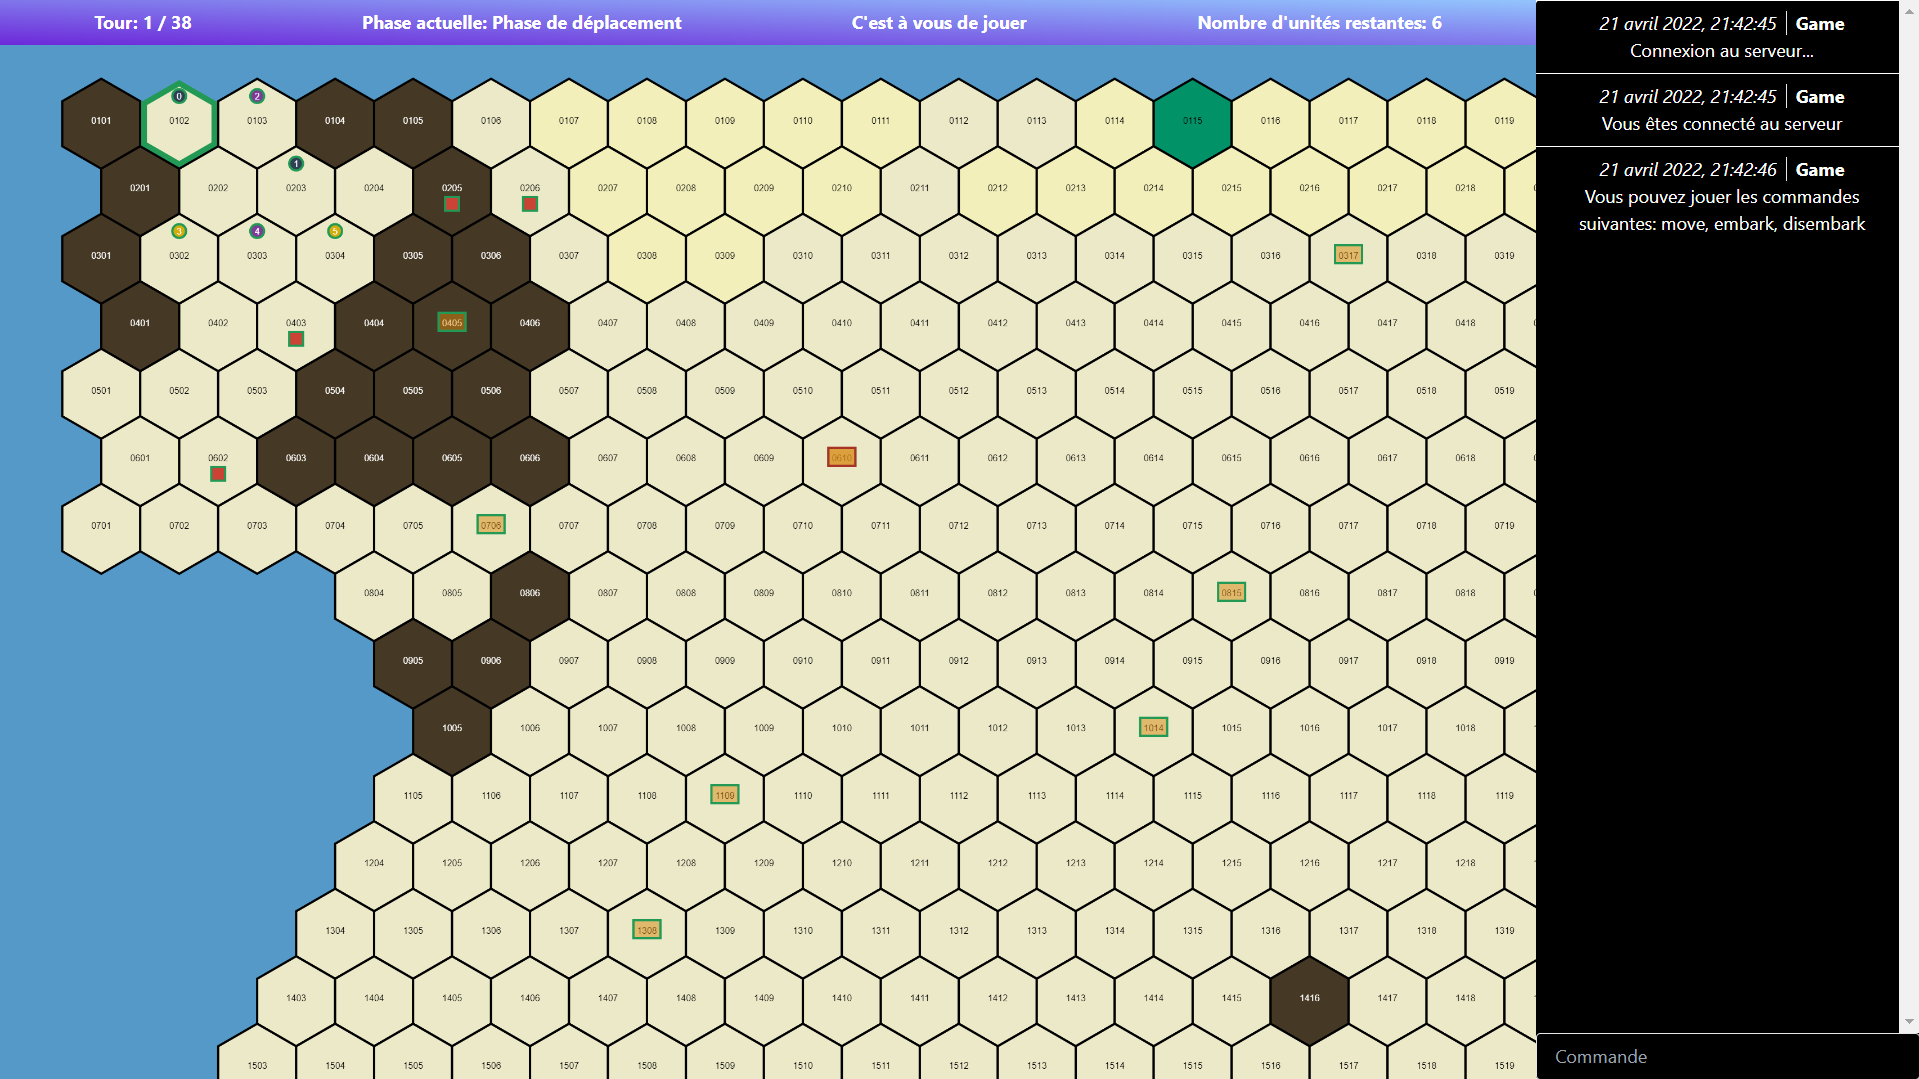
\includegraphics[scale=0.35]{data/plateau_du_jeu.png}
    \caption{Plateau du jeu Desert Fox}.
\end{figure}

En bas à gauche de la carte une légende explique les types de terrain et les types d'entités.\\

\begin{figure}[H]
    \centering
    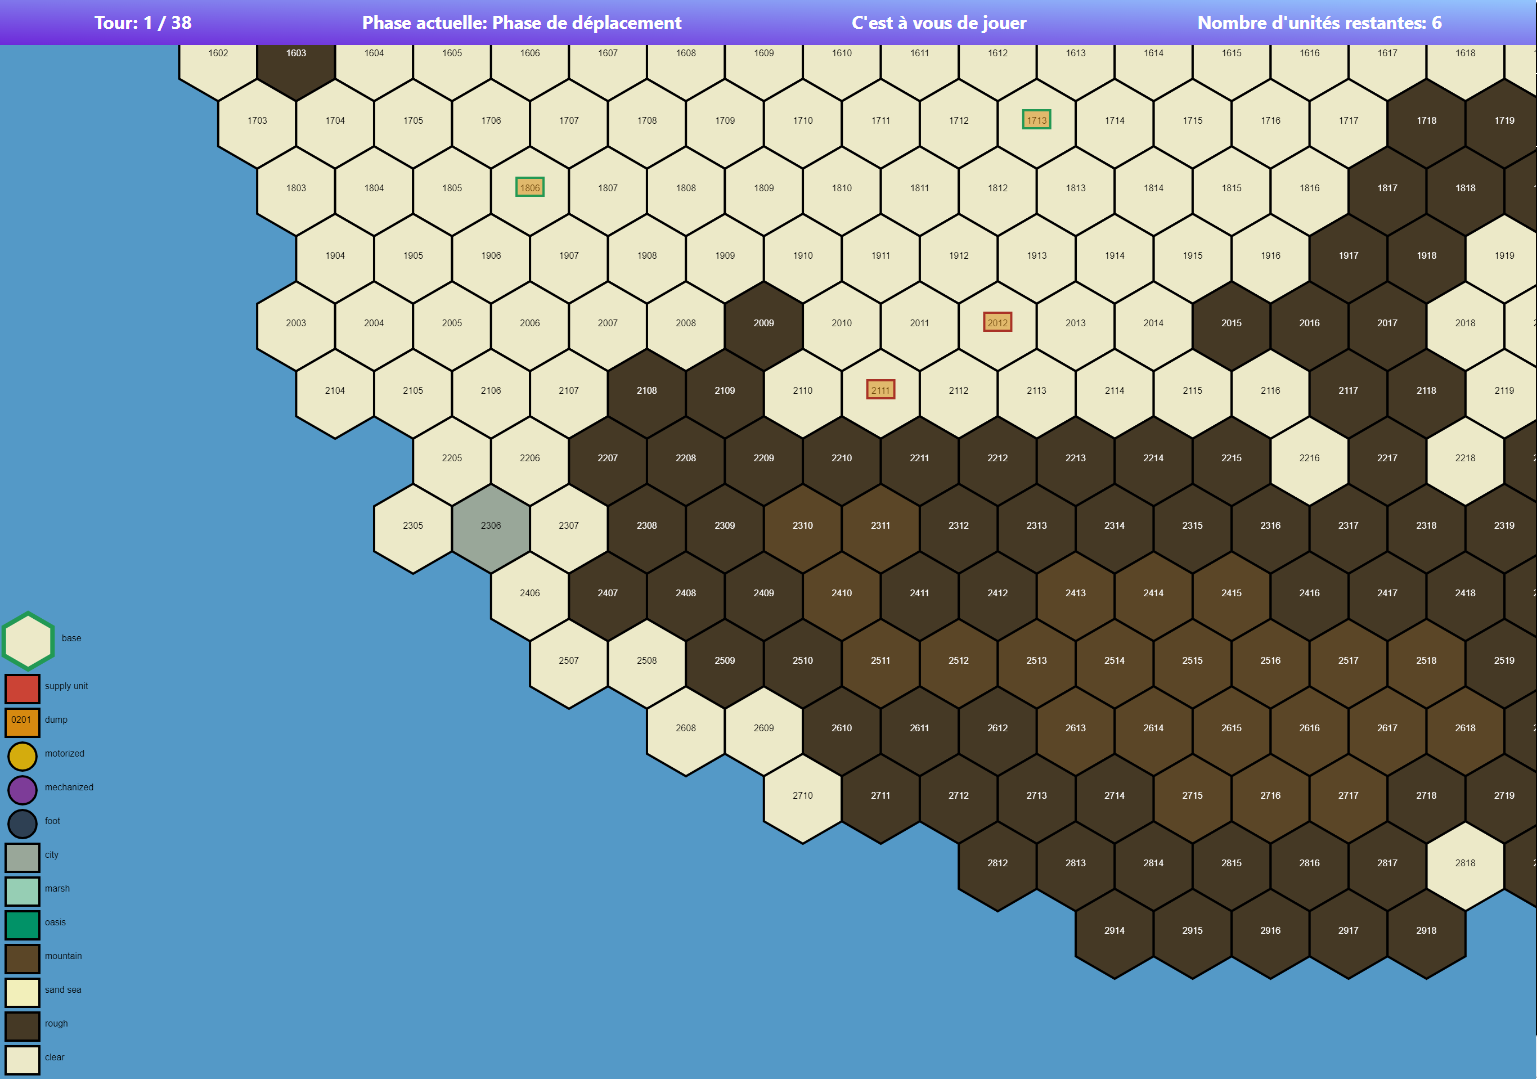
\includegraphics[scale=0.45]{data/Bas_de_map.png}
    \caption{Bas de la carte du jeu}.
\end{figure}
\begin{figure}[H]
    \centering
    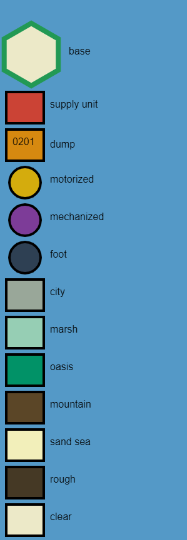
\includegraphics[scale=0.8]{data/Map_Legend.png}
    \caption{Légende de la carte du jeu}.
\end{figure}

Voici la page du joueur 1 qui peut jouer.\\
\begin{figure}[H]
    \centering
    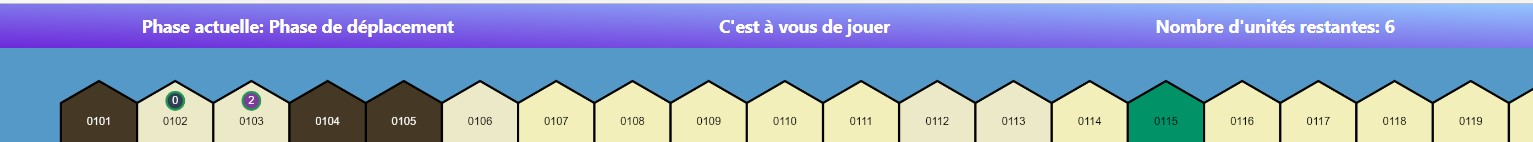
\includegraphics[scale=0.6]{data/player_1_acces.jpg}
    \caption{Barre d'information du joueur 1}.
\end{figure}

Voici la page du joueur 2 qui doit attendre l'adversaire de jouer.\\
\begin{figure}[H]
    \centering
    
\includegraphics[scale=0.6]{data/joueur_2.jpg}
    \caption{Barre d'information du joueur 2}.
\end{figure}

Le joueur qui peut jouer peut faire bouger son unité dans le terminal à droite de l'image.
Nous pouvons voir que l'unité 0 s'est déplacé de l'hexagone \lstinline{0102} à \lstinline{0206}. Le déplacement est valide, car on ne dépasse pas la capacité de mouvement de l'unité (MA).\\

\begin{figure}[H]
    \centering
    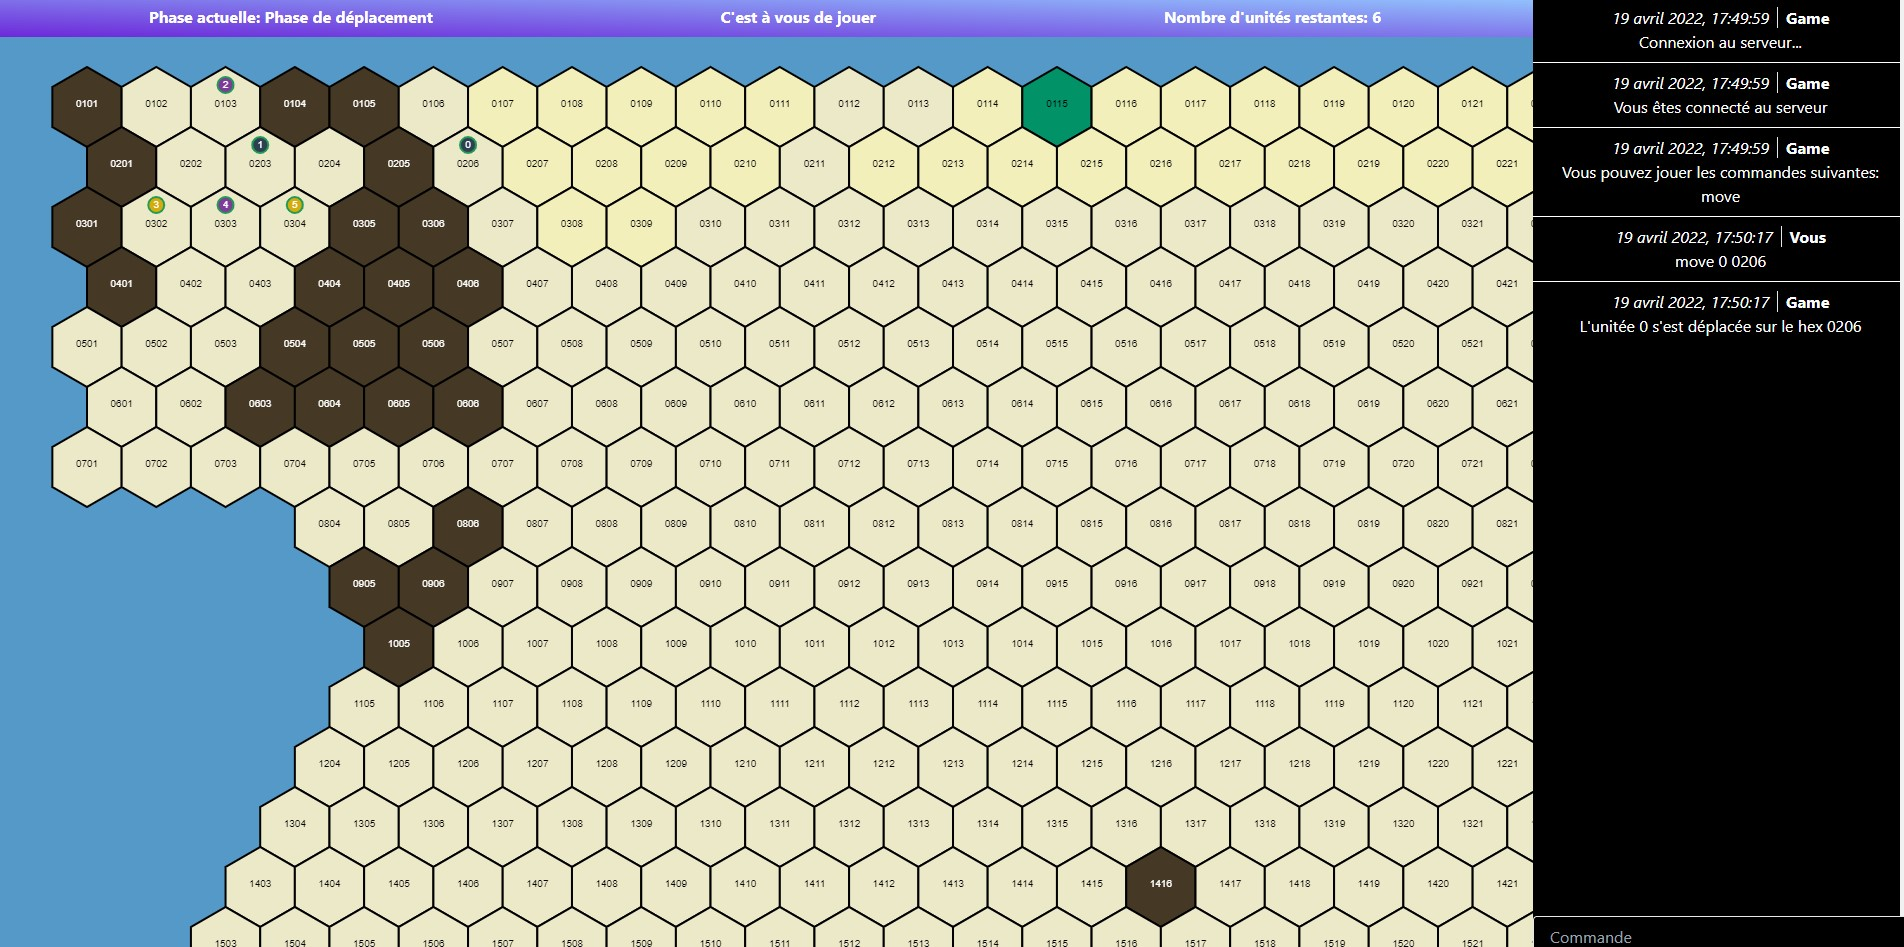
\includegraphics[scale=0.35]{data/move_unit_player_1.jpg}
    \caption{Mouvement de l'unité \lstinline{0} vers l'hexagone \lstinline{0206}}.
\end{figure}

Le joueur peut aussi utiliser une de ses unités de soutien pour bouger soit une unité de type {\tt foot} soit un dump.
Il peut faire cela avec la commande {\tt embark} qui prend en parametre l'identifiant de l'unité du soutien qui va embarquer, ainsi que l'identifiant de l'unité qui va etre embarquée. Voici un exemple :\\

\begin{figure}[H]
    \centering
    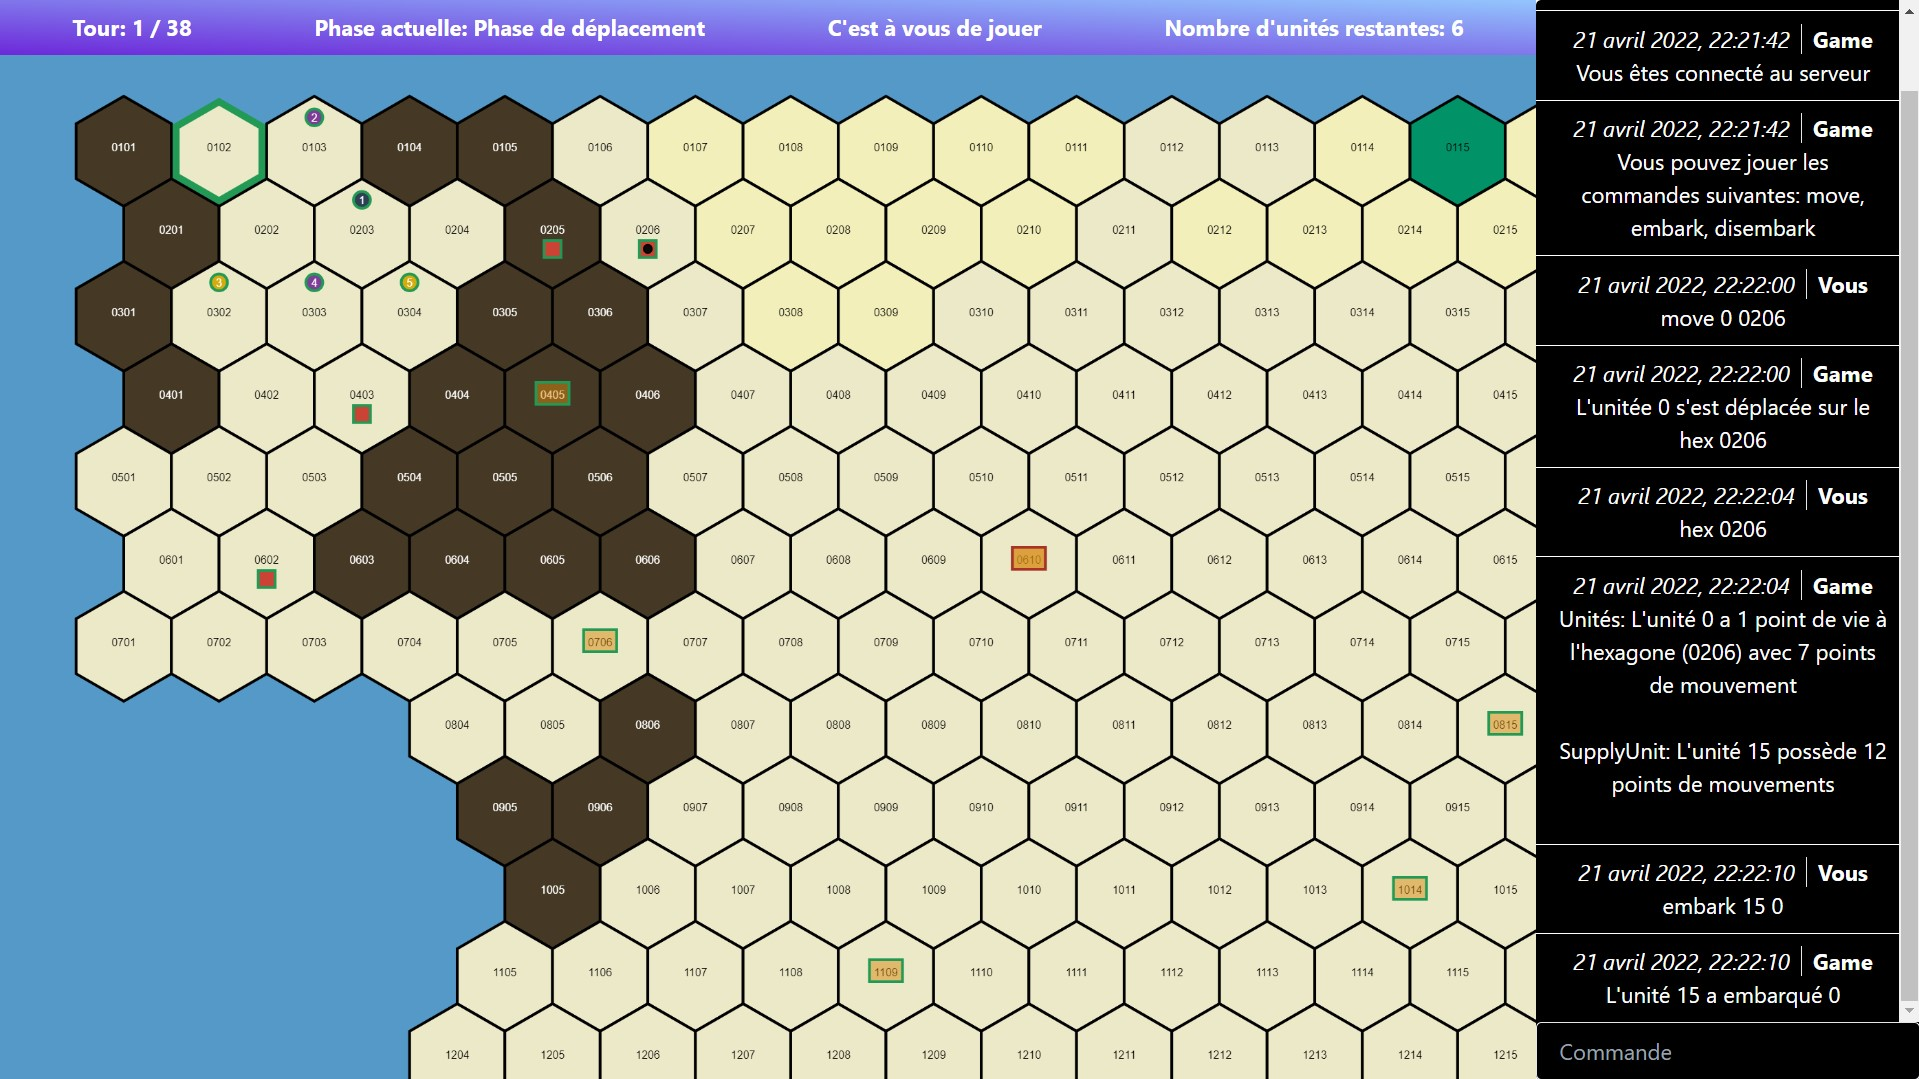
\includegraphics[scale=0.35]{data/Embark_command.jpg}
    \caption{Embarquement de l'unité \lstinline{0} dans l'unité de soutien  \lstinline{15}}.
\end{figure}

Il faut noter que l'unité qui est embarqué est inexistante dans la carte. Elle ne peut donc pas bouger elle meme, ni attaquer. Si l'unité du soutien a embarqué une unité, elle bougera avec elle. Dans la figure ci dessous nous pouvons voir que si nous embarquons un dump, qui est une entité qui ne peut pas bouger elle meme, nous pouvons la faire bouger avec l'unité de soutien. Ici nous la bougeons de l'hexagone \lstinline{0406} vers l'hexagone \lstinline{0407} \\

\begin{figure}[H]
    \centering
    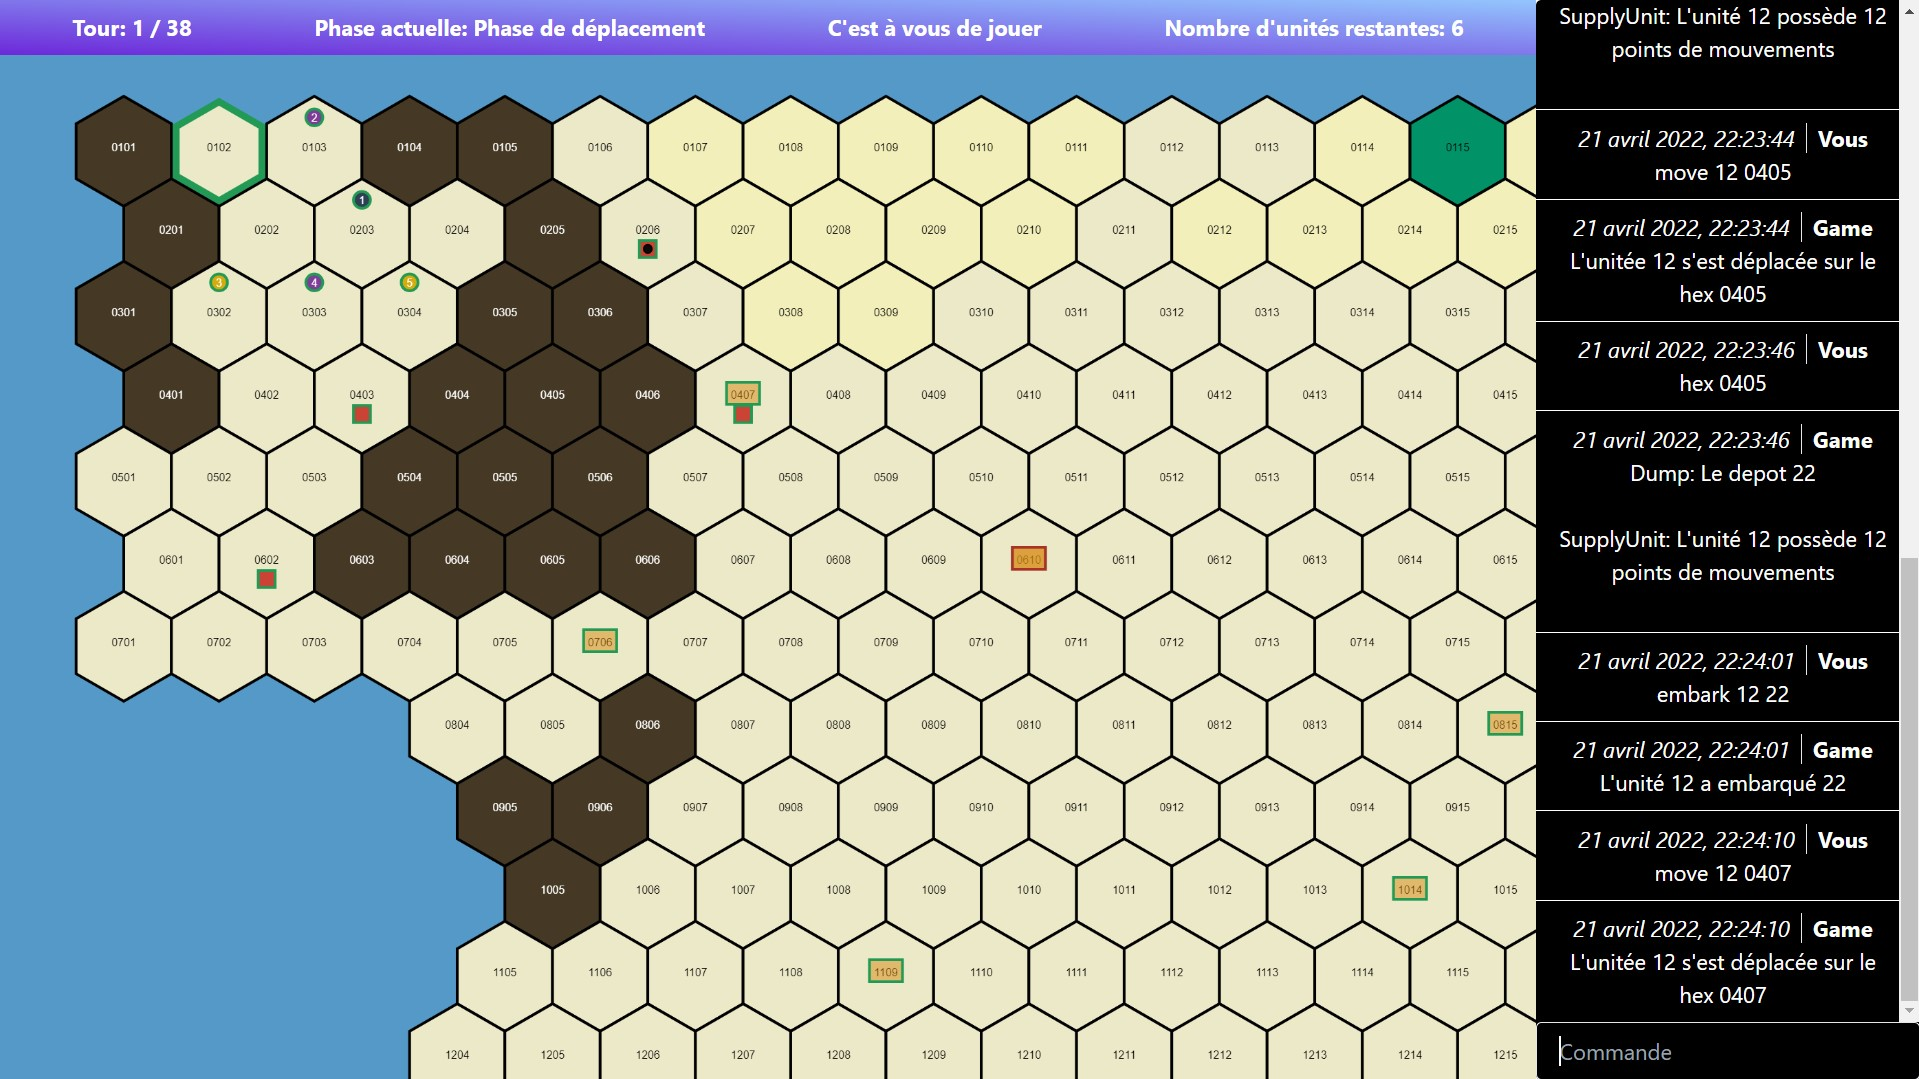
\includegraphics[scale=0.35]{data/Embark_dump.jpg}
    \caption{Embarquement du dump \lstinline{22} dans l'unité de soutien  \lstinline{12} suivi par un deplacement de l'unité du soutien à l'hexagone \lstinline{0407} (avec le dump)}.
\end{figure}

Afin de pouvoir reutiliser l'unité ou l'entité embarquée, nous devons utiliser la commande disembark, laquelle permet de debarquer cette dernière.
Dans la figure ci dessous nous pouvons voir que apres avoir bougé l'unité de soutien {\tt 15}, laquelle contient l'unité {\tt 0} et désembarquer, l'unité est dorénavant disponible pour un autre mouvement ou action. Elle est aussi affiché à nouveau dans la carte.\\

\begin{figure}[H]
    \centering
    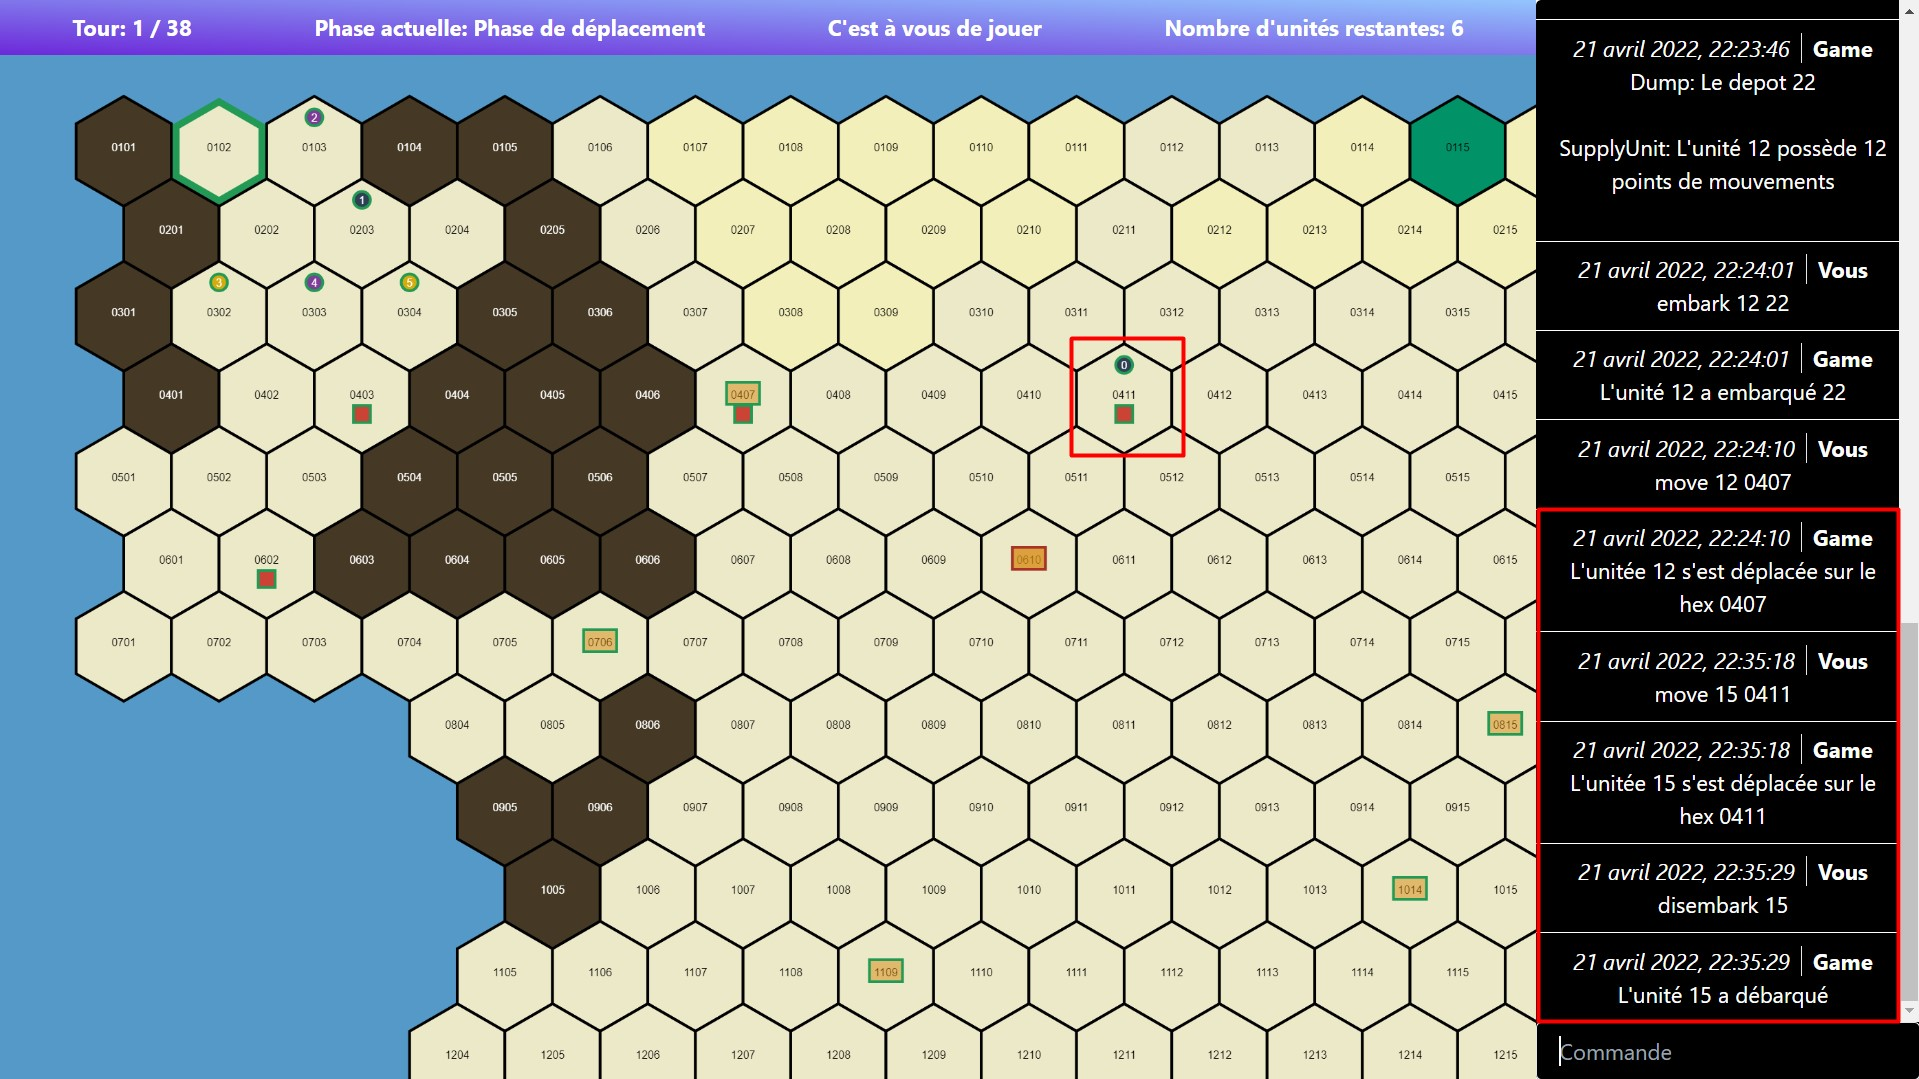
\includegraphics[scale=0.35]{data/Disembark.jpg}
    \caption{Mouvement de l'unité du soutien \lstinline{15}, laquelle contient l'unité \lstinline{0} à l'hexagone \lstinline{0411}, suivi du désembarquement de l'unité embarquée}.
\end{figure}

L'utilisateur peut aussi utiliser la commande {\tt attack} pour attaquer une unité adverse. Il faut noter que l'attaque est uniquement possible si l'unité est dans une case adjacente de l'unité adverse. Dans l'exemple ci dessous, nous pouvons voir que l'unité {\tt 5} \\

Le joueur peut afficher des informations concernant ses unités dans le terminal.
En tapant \og units \fg{}, le joueur à toutes ses unités présent avec le mouvement point et  les points de vies.
. Vous pouvez voir un exemple d'utilisation dans l'annexe a la figure \ref{fig:units_command}. \\




Quand le joueur a terminé son tour, il doit écrire dans le terminal \og done \fg{}. Le joueur ne pourra que communiquer par chat à l'adversaire et l'adversaire peuvent continuer à jouer. Voir figure \ref{fig:fin_tour}\\



Le joueur peut aussi afficher les entités, par exemple les unités, les bases, les dumps et les unités de soutien qui sont present dans une hexagone.
Cela est possible grace a la commande {\tt hex}, qui prend en parametre un identifiant d'hexagone.Voici un exemple :\\

\begin{figure}[H]
    \centering
    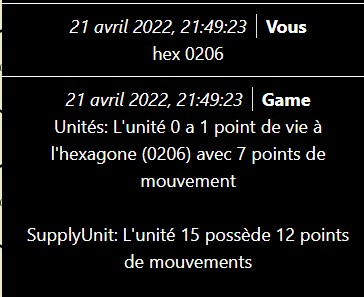
\includegraphics[scale=0.75]{data/hex_command.jpg}
    \caption{Utilisation de la commande hex}.
\end{figure}

Les deux joueurs peuvent communiquer ensemble  à l'aide du terminal, le joueur doit écrire au dans le terminal \og message \fg{} puis écrit son message.\\
\begin{figure}[H]
    \centering
    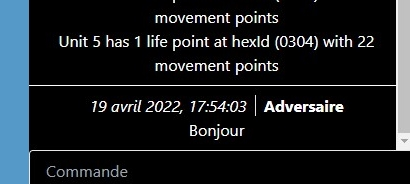
\includegraphics[scale=0.6]{data/chat.jpg}
    \caption{Communication entre deux joueurs}.
\end{figure}

Un message d'erreur s'affiche dans le terminal si le joueur écrit  des mauvaises commandes.
Par exemple, le joueur oublie les arguments, ou donne un mauvais hexagone.\\

\begin{figure}[H]
    \centering
    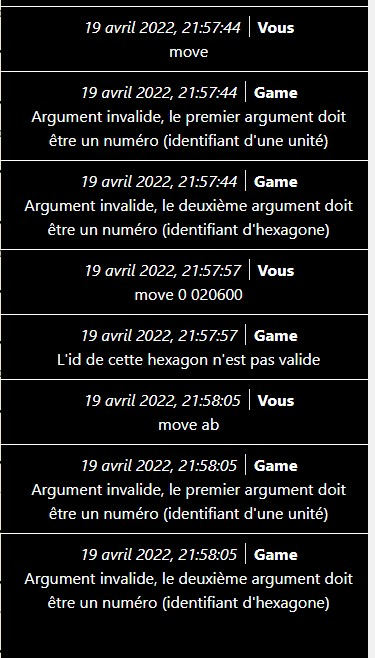
\includegraphics[scale=0.6]{data/erreur.jpg}
    \caption{Exemple de mauvaises commandes}.
\end{figure}


\newpage


\section{Architecture Logiciel}

Nous avons divisé notre modèle en deux grandes architectures, le serveur et les unités. 

\subsection{Architecture du serveur}

TODO: Expliquer l'architecture du serveur en détail, c'est-à-dire 2 listes: une de player et une de sockets, il y a une stateMachine qui gère les différents états du jeu,
le jeu est créé quand les 2 joueurs sont connectés, la carte est envoyée à  ce moment-là, quand une action est effectuée qui change la carte il faut renvoyer la carte

\subsection{Architecture des unités}

\begin{figure}[H]
    \centering
    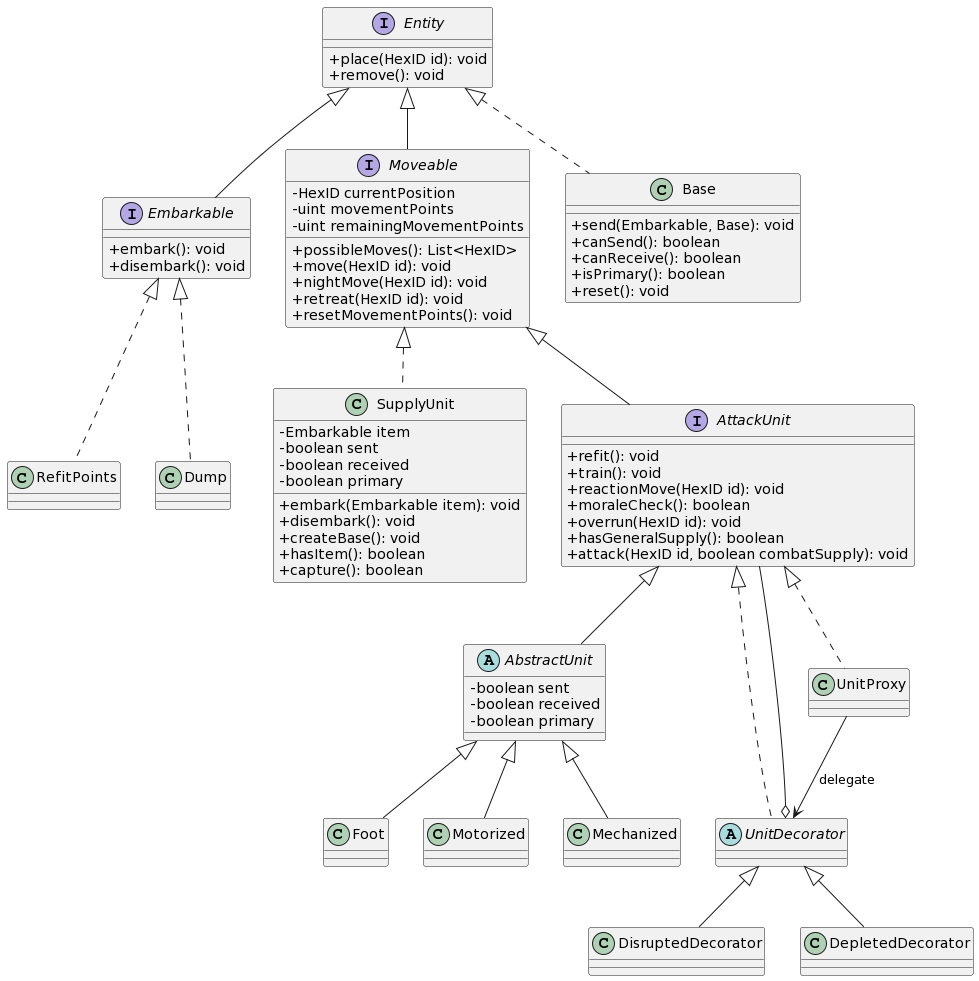
\includegraphics[scale=0.3]{data/uml_entityV4.png}
    \caption{Diagramme UML de l'objet \emph{Entity}}
    \label{fig:uml_entity}
\end{figure}

Nous avons fait le choix de réunir toutes les unités sous la même interface, ce qui nous permet d'avoir un seul type pour toutes les unités et donc de pouvoir faire des listes de ces entités dans la partie serveur.
Pour une meilleure factorisation on sépare les unités en deux, celles qui peuvent bouger (\lstinline{Moveable}) et les autres. Nous séparons de nouveau en unités de soutien et d'attaque. Pour assurer la maintenance du code et rajouter des fonctionnalités, nous avons utilisé deux designs patterns, le \lstinline{Decorator} et le \lstinline{Proxy}. Mais pour pouvoir utiliser ces patterns nous avions la contrainte suivante, il fallait que les deux patterns implémentent une interface comme montrer ci-dessous. Nous avons donc était forcé d'ajouter une interface intermédiaire (ici \lstinline{AttackUnit}) pour pouvoir les implémenter. Le décorateur nous permet de changer le comportement des unités dynamiquement sans à avoir à changer toutes les classes qui étendent \lstinline{AbstractUnit}. Mais l'utilisation de ce pattern conduit à un problème, on peut appliquer un décorateur à un objet déjà décorer un nombre de fois infinie. Ce qui nous amène donc à utiliser un \lstinline{Proxy} qui permet de contrôler l'utilisation du décorateur. 

Toute la démonstration précédente était notre réflexion lors de la conception de l'architecture. Mais nous avons implémenté l'attaque en dernier, il est donc possible que les patterns énoncés ne soient pas présents dans le code.

\begin{figure}[H]
    \centering
    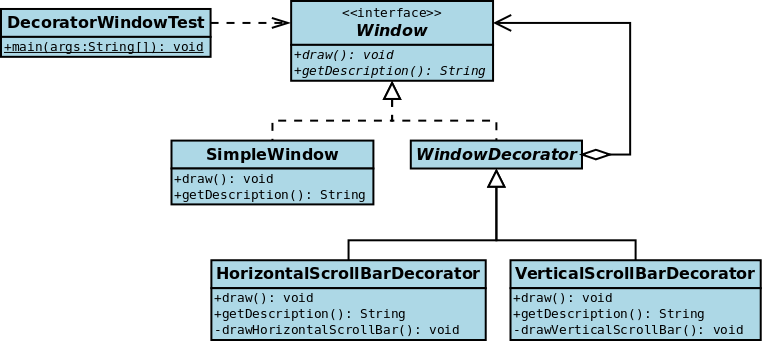
\includegraphics[scale=0.3]{data/UML_Decorator_Pattern_Exmple.png}
    \caption{Exemple Wikipedia à rajouter dans bibliographie}
\end{figure}

\begin{figure}[H]
    \centering
    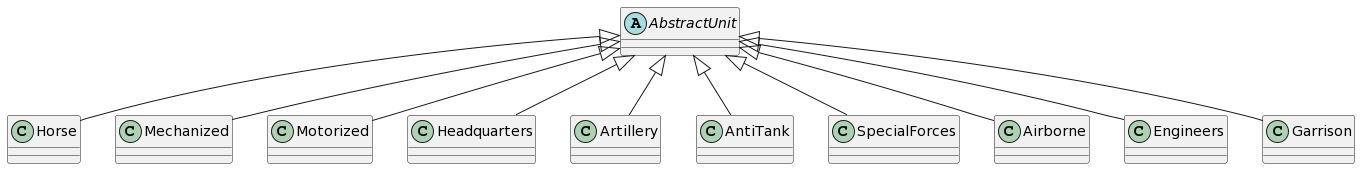
\includegraphics[scale=0.3]{data/uml_abstract_unit.png}
    \caption{Diagramme UML des unités}
\end{figure}

Dans les règles ils existent toutes les unités d'attaque qui se trouvent ci-dessus. Comme nous avions un temps limité nous avons décidé de ne pas toutes les implémenter car même si certaines ont un comportement différent le travail aurait été chronophage et donc nous avons privilégié des aspects plus importants du projet. On peut trouver les unités d'attaque choisies dans le diagramme \ref{fig:uml_entity} (Foot, Mechanized, Motorized).

\section{Technologies}

\subsection{Service d'hébergement}

Pour le service d'hébergement nous avons utilisé le GitLab du Cremi comme demandé dans les consignes. Nous avons paramétré les pipelines pour qu'à chaques commits il effectue les tests automatiquement pour aider à ne pas faire des commits complètement erronés. Concernant les branches nous avons divisé le dépôt en quatre:
\begin{itemize}
    \item main
    \item dev
    \item backend
    \item frontend
\end{itemize}

Le principe est que l'on développe sur les branches correspondantes (\lstinline{frontend} et \lstinline{backend}), que l'on fusionne ces deux dernières sur la branche \lstinline{dev} pour vérifier si tout se passe bien et enfin mettre à jour le main pour avoir une version stable. Cela nous paraissait le plus logique sauf que l'on s'est vite rendu compte que ce n'était pas le moyen le plus optimisé de travailler car lorsqu'on travaille sur la même chose sur le \lstinline{backend} et le \lstinline{frontend} cela produisait divers bugs lorsqu'on réunissait les deux branches. Il aurait sûrement plutôt réfléchir en features et donc créer une branche pour chaque tâche.

\subsection{Langage de programmation}

Nous avons choisi comme langage de programmation \lstinline{TypeScript} pour le \lstinline{backend} et le \lstinline{frontend}. En effet en ayant la même technologie pour tout le projet cela rend la communication beaucoup plus simple entre les deux côtés. On aurait aussi pu utiliser \lstinline{JavaScript} mais une surcouche de typage nous permet de sécuriser la production du code. Enfin ce choix nous a laissé la liberté de ne pas faire que de la programmation objet, par exemple le \lstinline{frontend} est en majorité de la programmation impérative.

\subsection{Communication client-serveur}

Au départ nous étions parti sur une architecture avec un serveur web qui communiquait avec les clients grâce à des requêtes web HTTP.

Malheureusement cette architecture n'était pas adaptée pour un jeu de ce type puisque au moment où un joueur joue un coup, l'autre joueur doit être notifié de ce changement. Or si on utilise un serveur web HTTP le client devrait faire une requête au serveur pour être mis au courant, ce qui n'est pas pratique.

Pour un changement en direct sans faire une boucle de requêtes continuelles, il faudrait un système où le serveur peut envoyer un message au client sans requête au préalable.

C'est pour cela qu'une architecture avec des web sockets a été la solution que nous avons choisie.
Cette architecture permet d'envoyer des messages ou des données aux clients sans requête préalable.


\begin{figure}[H]
    \centering
    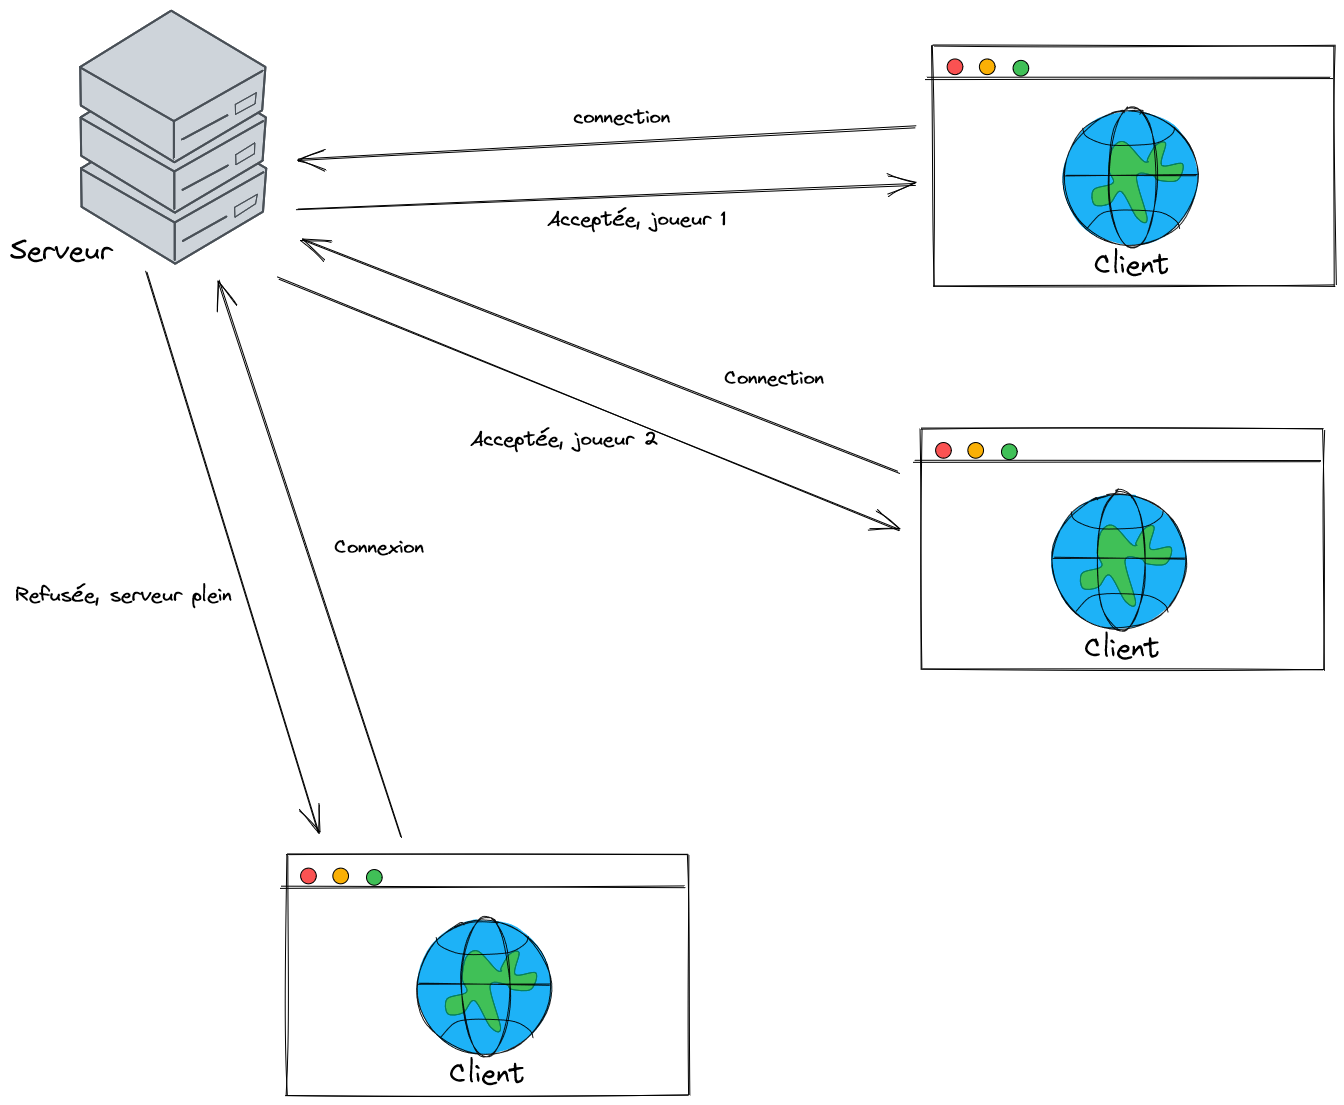
\includegraphics[scale=0.25]{data/reseau_initialisation.png}
    \caption{Phase de connexion des joueurs au serveur}
\end{figure}

Ici on peut voir la première phase du serveur qui permet d'enregistrer les connexions des deux joueurs pour créer une partie.

La partie de connexion est gérée par la bibliothèque {\tt socket-io} que nous utilisons pour le serveur et le client. C'est l'avantage essentiel d'utiliser la même technologie sur le backend et le frontend.

Dans le serveur, nous sauvegardons les sockets qui se connectent au serveur. La limite est de 2 puisqu'il y a 2 joueurs maximum. Quand les 2 joueurs sont bien connectés, la partie est pleine. S'il y en a déjà 2 lors d'une connexion d'un troisième socket, alors la connexion de la troisième est refusée et cette dernière reçoit un code d'erreur, {\tt full}, que le frontend de ce socket va afficher à l'utilisateur.
Si un autre joueur essaie de se connecter, alors le socket n'est pas sauvegardé dans le serveur et elle est déconnectée, il reçoit également une erreur, {\tt full}, qui va s'afficher dans le terminal.

Une fois les deux joueurs créés et la partie initialisée, la carte est envoyée aux deux joueurs pour l'affichage. Voir ci-dessous \ref{reseau_carte}.

\begin{figure}[H]
    \centering
    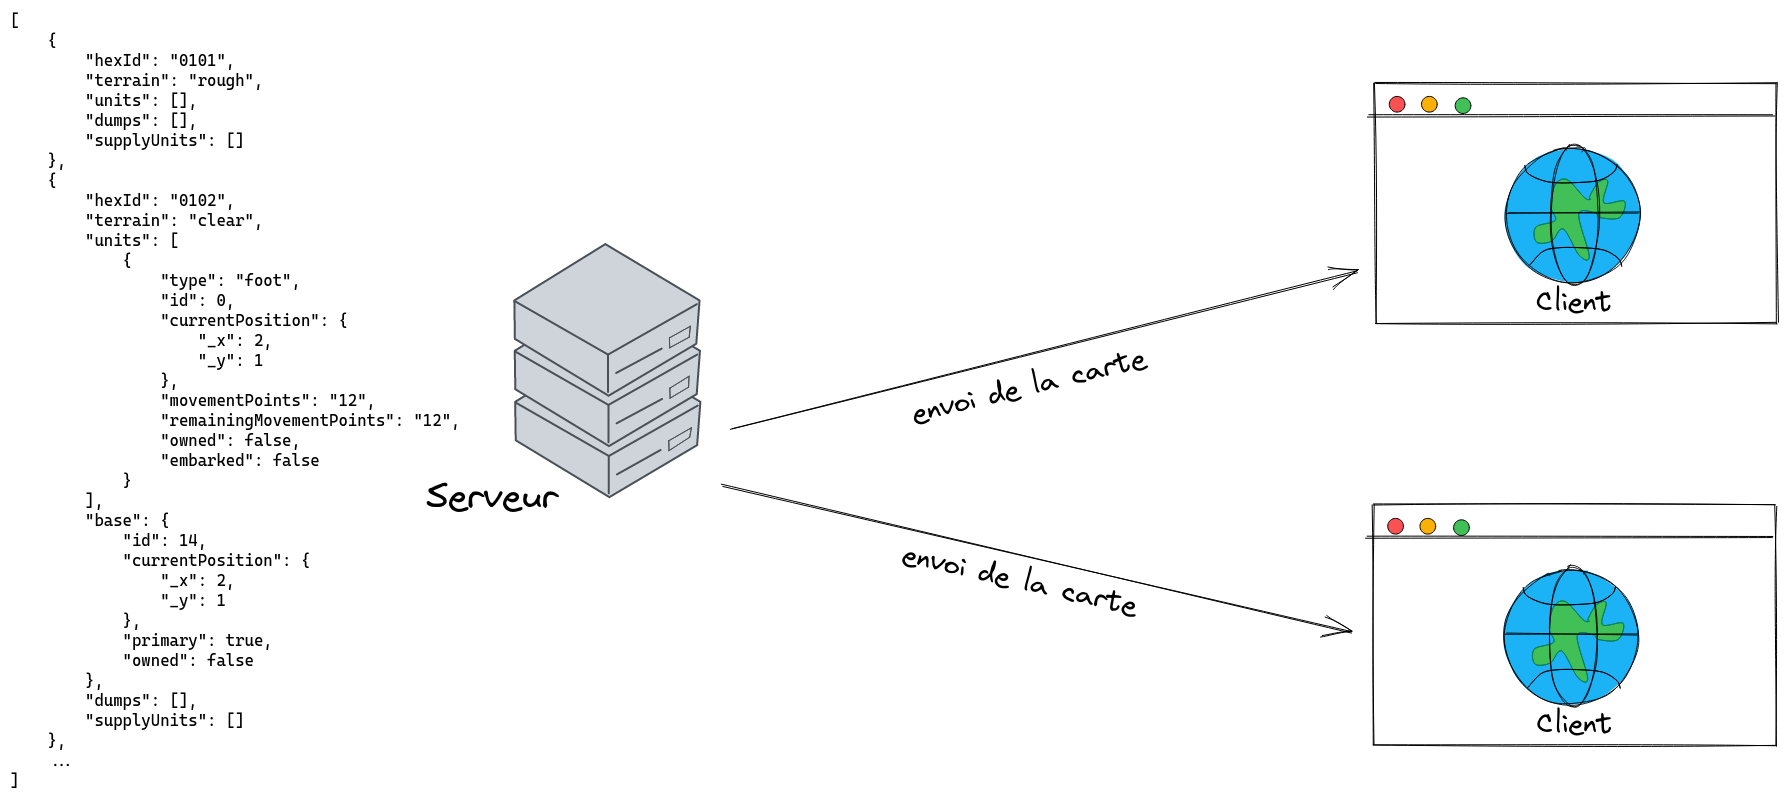
\includegraphics[scale=0.25]{data/reseau_map.png}
    \caption{Phase de connexion des joueurs au serveur}
    \label{reseau_carte}
\end{figure}

Le code à gauche du serveur est le début du {\tt JSON} original envoyé à chaque client.
On peut voir comment il est constitué : c'est un tableau d'objets. Chacun de ces objets représente une case.
Chaque case possède un ``id``, un identifiant, ainsi qu'un ``terrain`` qui décrit son type de terrain.
Il possède aussi 3 aux champs, ``units``, ``dumps`` et ``supplyUnits`` qui sont des tableaux d'objets.
Comme leurs noms l'indique ces objets représentent des tableaux d'unités, de dépôts ou d'unités de ravitaillement.

À partir de ce moment-là, le moteur graphique du jeu est chargé de dessiner la carte reçue en JSON.
L'action \ref{reseau_carte} se répète à chaque changement de la carte dans le jeu.


Les phases vont donc s'enchaîner jusqu'à ce qu'une action d'un joueur soit requise.

\begin{figure}[H]
    \centering
    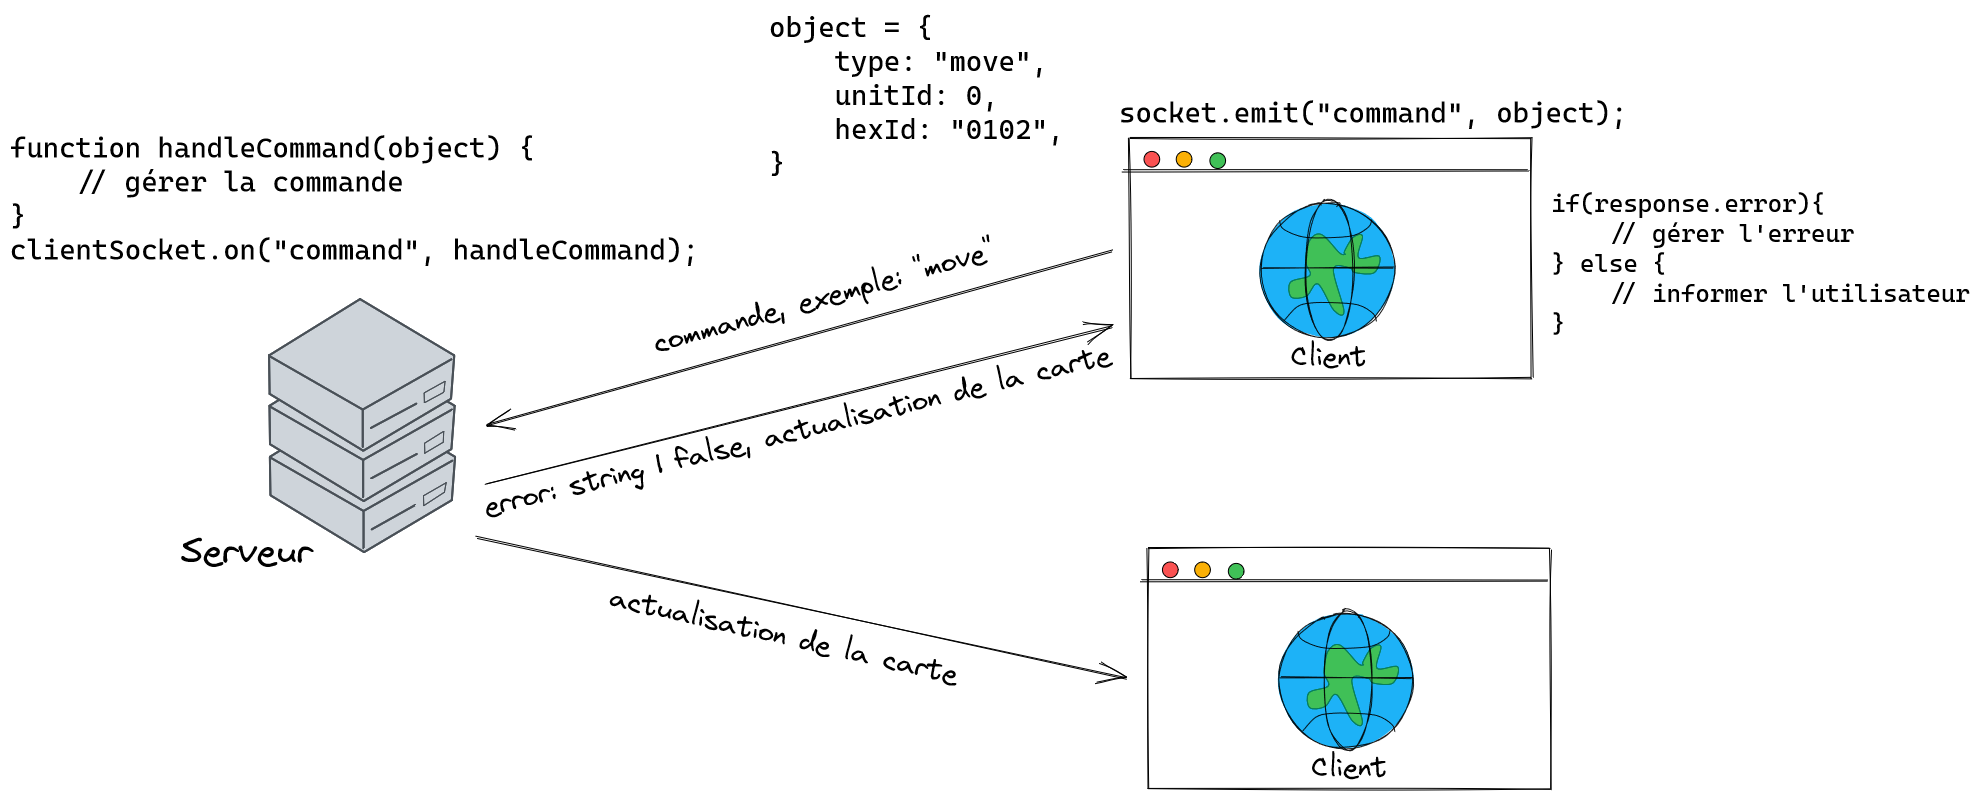
\includegraphics[scale=0.25]{data/reseau_commande.png}
    \caption{Phase de jeu, exemple de commande {\tt move}}
\end{figure}

TODO

La partie s'exécute normalement jusqu'à la fin.

\subsection{}

Vue.js

\subsection{Test}

Pour les tests nous avons utilisé Mocha qui est un cadre de test JavaScript pour les programmes Node.js. Nous testons le backend et les communications des sockets parce qu'il est compliqué de tester l'affichage. Nous avons réalisé des tests unitaires, la couverture du code est aussi vérifiée grâce à NYC qui est un framework compatible avec Mocha. Nous y reviendrons plus tard dans une partie dédiée.

\subsection{Interface graphique}

Dans le sujet il était indiqué que l'on n'était pas dans l'obligation de faire une interface graphique. Mais afficher un hexagone dans un terminal est compliqué et la moitié de la carte donnée en exemple est de dimensions 32*29 cases, ce qui aurait donné un rendu illisible. Nous avons donc fait le choix de faire une interface graphique. Pour afficher la carte nous avons testé plusieurs bibliothèques et choisis \lstinline{P5.js} pour plusieurs raisons, la documentation est claire et la bibliothèque est plutôt populaire ce qui facilite les recherches lors de problèmes d'implantation (tutoriels, stackoverflow...).

Notre approche pour afficher la carte est de la dessiner à chaque changement dans le \lstinline{backend} (exemple: un move). La première raison à cette tactique est de rendre l'affichage plus facile vu que ce n'est pas la priorité du sujet. Et si nous avions dû faire un affichage dynamique il aurait fallu créer des objets pour sauvegarder la position des unités dans chaque case. Ce qui implique aussi une duplication de la logique du \lstinline{backend}, nous avons voulu éviter ça. Ici le \lstinline{backend} envoie des données, on les parse et on les affiche.

Pour dessiner les hexagones de la map nous avons cherché des algorithmes pour ne pas avoir à les développer nous-mêmes mais nous n'avons trouvé que des affichages comme suivant.

\begin{figure}[H]
    \centering
    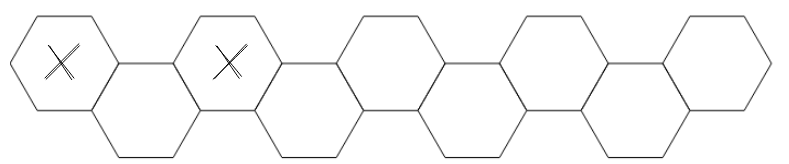
\includegraphics[scale=0.3]{data/hexmap_exemple.png}
    \caption{Une ligne d'hexagones}
\end{figure}
% source https://eperezcosano.github.io/hex-grid

 Le problème de ce genre d'affichage est que deux cases sur la même ligne (avec les croix) ne se touchent pas. On ne peut donc pas faire de déplacement d'unité. Nous avons alors fait nos propres méthodes pour avoir un hexagone dans l'autre sens (avec la pointe vers le haut) et qui est donc adjacente à ses six voisins comme suit. Pour cela on calcule les points grâce au cercle trigonométrique.
 
\begin{figure}[H]
    \centering
    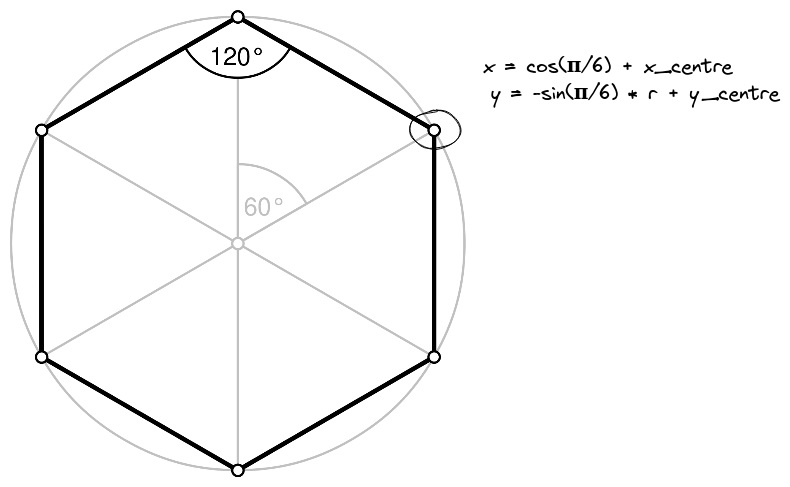
\includegraphics[scale=0.3]{data/hexagon.png}
    \caption{Les étapes pour dessiner un hexagone}
\end{figure}

 On peut aussi mettre six unités d'attaque dans une case, on réutilise donc le calcul de ces points pour faire la moyenne par rapport au centre. On se retrouve donc avec une unité dans chaque coin de l'hexagone. Ce qui donne le résultat suivant.
 
\begin{figure}[H]
    \centering
    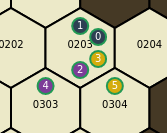
\includegraphics[scale=.7]{data/hexagon_with_units.png}
    \caption{Affichage hexagone avec des unités}
\end{figure}



\newenvironment{mytest}[4]
{
    \begin{center}
        \centering
        \begin{tabular}[h]{|m{4cm}|m{12cm}|}
            \hline
            \rowcolor[HTML]{F8B400}
            \textbf{But}    & #1 \\
            \hline
            \hline
            \rowcolor[HTML]{F7F7F7}
            Entrée          & #2 \\
            \hline
            \rowcolor[HTML]{F7F7F7}
            Scénario        & #3 \\
            \hline
            \rowcolor[HTML]{F7F7F7}
            Analyse du test & #4 \\
            \hline
        \end{tabular}
    \end{center}
}

\section{Nos tests}
Nous avons mis en place divers outils pour contrôler notre implémentation :
\begin{itemize}
    \item Chaque {\tt commit} sera vérifier par des pipelines de {\tt GitLab}. Cet outil compile le code proposé sur une machine afin de voir si le code suggérer n'a aucune erreur de compilation.
    \item L'implémentation de notre {\tt backend} est contrôlé par le framework {\tt NYC}. Nos tests sont surveillés par le framework et nous donne le résultat de {\tt coverage} pour chaque fichier testé.
\end{itemize}

\subsection{Test unitaire}

\subsubsection{Vérification des fichiers dans le fichier {\tt src}}

\mytest
{Vérifier si les fichiers possède le bon format (\texttt{.ts}) dans le dossier \texttt{src/main}}
{Un ensemble de fichiers}
{En cas de mauvais format dans le dossier, on affiche les fichiers qui ne respectent pas le format \texttt{.ts}}
{Parcours d'un dossier en ajoutant dans une liste les fichiers qui ne respecte pas la condition}

\mytest
{Vérifier si les fichiers possède le bon format (\texttt{.ts} ou \texttt{.json}) dans le dossier \texttt{src/test}}
{Un ensemble de fichiers}
{En cas de mauvais format dans le dossier, on affiche les fichiers qui ne respectent pas le format \texttt{.ts} ou \texttt{.json}}
{Parcours d'un dossier en ajoutant dans une liste les fichiers qui ne respecte pas la condition}

\mytest
{Chaque fichier possède une classe doit commencer par une majuscule dans le dossier \texttt{src/main}}
{Un ensemble de fichiers}
{En cas de non-respect des consignes, on affiche les fichiers qui ne respectent la capitalisation de la première lettre}
{On ajoute dans une liste les fichiers qui ne respecte pas la condition (parcours d'un dossier + manipulation de chaîne de caractère pour récupérer la première}

\subsubsection{Vérification de la carte du jeu}

\mytest
{Vérification de l'emplacement d'une case d'hexagone \#1}
{Identifiant d'une vraie case d'hexagone}
{Si l'identifiant n'est pas sur la carte du jeu, signalez cette case}
{Vérifie l'identifiant dans une table de hachage}

\mytest
{Vérification de l'emplacement d'une case d'hexagone \#2}
{Identifiant d'une fausse case d'hexagone}
{Si l'identifiant est inclus sur la carte du jeu, signalez cette case}
{Vérifie l'identifiant dans une table de hachage}

\subsubsection{Vérification du serveur {\tt socket}}

\mytest
{Vérification si le port du client est stocké correctement}
{Un entier représentant le port du client}
{En cas d'une inégalité entre le port du client et le port enregistré pour le serveur socket, nous levons une exception}
{On vérifie avec une comparaison entre deux entiers}

\mytest
{Vérification si le port du serveur est stocké correctement}
{Un entier représentant le port du serveur}
{En cas d'une inégalité entre le port du serveur et le port enregistré pour le serveur socket, nous levons une exception}
{On vérifie avec une comparaison entre deux entiers}

\mytest
{Vérification de la limite de joueurs dans une partie (2 joueurs maximum)}
{La connexion d'un joueur}
{En cas de connexion d'un troisième joueur, une exception est levée}
{Avant de vérifier la connexion d'un troisième joueur, nous attendons 500 millisecondes}

\mytest
{Vérification du lancement de la partie}
{Une instance du \texttt{serveur}}
{Avec notre instance du serveur, on essaye de récupérer le jeu, si ce n'est pas le cas, on lève une exception}
{On vérifie l'instance du jeu avec l'instance du serveur}

\mytest
{Vérification du joueur \#1 dans la partie}
{Une instance du \texttt{serveur}}
{Si le joueur \#1 n'est pas accessible via l'instance du jeu, nous levons une exception}
{On vérifie dans l'instance du jeu qui est accessible à partir de l'instance du serveur}

\mytest
{Vérification du joueur \#2 dans la partie}
{Une instance du \texttt{serveur}}
{Si le joueur \#2 n'est pas accessible via l'instance du jeu, nous levons une exception}
{On vérifie dans l'instance du jeu qui est accessible à partir de l'instance du serveur}

\mytest
{Vérification de l'identifiant du socket du joueur \#1}
{Une instance du \texttt{serveur}}
{
    \begin{itemize}
        \item Le joueur \#1 possède le socket du joueur \#2 $\rightarrow$ exception
        \item Le jeu ne possède pas le bon identifiant du joueur \#1 $\rightarrow$ exception
    \end{itemize}
}
{On récupère les identifiants des différents joueurs dans l'instance du jeu (accessible à partir de l'instance du serveur)}

\mytest
{Vérification de l'identifiant du socket du joueur \#2}
{Une instance du \texttt{serveur}}
{
    \begin{itemize}
        \item Le joueur \#2 possède le socket du joueur \#1 $\rightarrow$ exception
        \item Le jeu ne possède pas le bon identifiant du joueur \#2 $\rightarrow$ exception
    \end{itemize}
}
{On récupère les identifiants des différents joueurs dans l'instance du jeu (accessible à partir de l'instance du serveur)}

\mytest
{Vérification de la fin de partie lors de la déconnexion d'un joueur}
{Une instance du serveur et le socket d'un joueur}
{Si le jeu est accessible à partir du joueur déconnecté, alors nous levons une exception}
{On vérifie dans l'instance du serveur, si on peut récupérer le jeu}

\mytest
{Vérifier si le dernier joueur reste connecté au jeu malgré la déconnexion de son adversaire}
{Une instance du \texttt{serveur}}
{On doit retrouver un joueur dans l'instance du \texttt{serveur}, sinon on lève une exception}
{
    \begin{itemize}
        \item On vérifie la longueur de la liste des joueurs
        \item Le dernier joueur possède le bon identifiant
        \item On vérifie si le joueur a bien été supprimé de la liste des joueurs
    \end{itemize}
}

\mytest
{Vérification du redémarrage du jeu lors de la connexion du premier joueur}
{Socket du premier joueur et une instance du \texttt{serveur}}
{Si le joueur ne reçoit pas une instance du jeu, nous levons une exception}
{Lors de la connexion du joueur, il reçoit le jeu}

\mytest
{Vérification du redémarrage du jeu lors de la connexion du deuxième joueur}
{Socket du deuxième joueur et une instance du \texttt{serveur}}
{Si le joueur ne reçoit pas une instance du jeu, nous levons une exception}
{Lors de la connexion du joueur, il reçoit le jeu}

\mytest
{Vérification de la communication entre le serveur et le client (joueur)}
{Le socket d'un joueur}
{Le joueur envoie un message \texttt{ping} au serveur. Il sera immédiatement répondu par le serveur par un message \texttt{pong}}
{Le client envoie un message et attends une réponse du serveur.}

\mytest
{Vérification de la communication entre le serveur et le client}
{Les sockets des deux joueurs}
{On vérifie si un message part du point A au point B, sinon on lève une exception}
{Le joueur \#1 envoie un message \quotes{\texttt{Hello world}} et on vérifie si le joueur \#2 a reçu le message}

\subsubsection{Vérification de la machine d'état}
\mytest
{Vérification de l'instanciation de la machine d'état}
{Les spécificités nécessaires pour démarrer la machine d'état, dont les phases}
{Nous affichons une erreur si la machine n'est pas bien instanciée}
{Vérifie si l'état actuel est l'état initial}

\mytest
{Vérification du redémarrage de la machine d'état}
{La machine d'état lancée dans le test précédent}
{Nous affichons une erreur incluant l'état actuel et l'état attendu si la machine n'est pas bien redémarrée}
{Vérifie si l'état actuel est bien l'état initial}

\mytest
{Vérification des transitions de la machine d'état}
{La machine d'état lancée dans le premier test de cette section}
{Nous affichons une erreur incluant l'état actuel et l'état attendu si l'état n'est pas bien changé}
{Vérifie après chaque appel au changement de l'état actuel de la machine d'état si ce dernier est correct}

\mytest
{Vérification du compteur de tours}
{La machine d'état lancée dans le premier test de cette section}
{Nous affichons une erreur incluant l'état actuel et l'état attendu si l'état actuel est erroné}
{Vérifie si après une série de changements de phases, la machine d'état met bien à jour le nombre du tour actuel}

\mytest
{Vérification du compteur de tours}
{La machine d'état lancée dans le premier test de cette section}
{Nous affichons une erreur incluant le nombre de tours actuels et le nombre de tours attendu si le nombre de tours est incorrect}
{Vérifie si après une série de changements de phases, la machine d'état met bien à jour le nombre du tour actuel}

\mytest
{Vérification le changement de phases pendant un tour}
{La machine d'état lancée dans le premier test de cette section}
{Nous affichons une erreur incluant l'état actuel et l'état attendu si l'état actuel est erroné}
{Vérifie si après une série de changements de phases égale au nombre totale de phases dans le jeu, l'état de la machine d'état est initiale}

\subsubsection{Vérification de l'instance du jeu}

\mytest
{Vérification de l'instanciation du serveur du jeu}
{L'adresse du client, le port du serveur et l'instance de la machine d'état}
{Nous affichons une erreur si l'instance du jeu n'est pas bien instanciée}
{Vérifie si le serveur du jeu se lance sans erreurs}

\mytest
{Vérification de l'instanciation du joueur 1}
{Le port du serveur pour que nous puisions connecter le premier joueur}
{Nous affichons une erreur si le premier joueur n'est pas bien connecté}
{Vérifie si le premier joueur se connecte sans erreur}

\mytest
{Vérification de l'instanciation du joueur 2}
{Le port du serveur pour que nous puisions connecter le deuxième joueur}
{Nous affichons une erreur si le deuxième joueur n'est pas bien connecté}
{Vérifie si le deuxième joueur se connecte sans erreur}

\mytest
{Vérification du lancement du jeu}
{Le serveur du jeu}
{Nous affichons une erreur si le jeu n'est pas bien lancé, ainsi que si les deux joueurs sont bien connectés ou pas}
{Vérifie si le jeu se lance sans erreur après la connexion des 2 joueurs}

\mytest
{Vérification de la commande {\tt units} tant que premier joueur}
{La {\tt socket} du premier joueur}
{Nous affichons une erreur si le premier joueur n'a pas reçu le bon résultat en exécutant la commande {\tt units} ainsi que le nombre correct et actuel si ce dernier est incorrect}
{Vérifie si le premier joueur reçoit bien ses unités avec leurs spécificités après l'appel à la commande {\tt units}}

\mytest
{Vérification de la commande {\tt units} tant que deuxième joueur}
{La {\tt socket} du deuxième joueur}
{Nous affichons une erreur si le deuxième joueur n'a pas reçu le bon résultat en exécutant la commande {\tt units} ainsi que le nombre correct et actuel si ce dernier est incorrect}
{Vérifie si le deuxième joueur reçoit bien ses unités avec leurs spécificités après l'appel à la commande {\tt units}}

\mytest
{Vérification de la commande {\tt move} tant que premier joueur avec des arguments corrects}
{La {\tt socket} du premier joueur, ainsi que les arguments corrects pour la commande {\tt move}}
{Nous affichons une erreur si le premier joueur n'a pas bien effectué {\tt move} ainsi que l'erreur correspondante}
{Vérifie si le premier joueur effectue correctement le mouvement après l'appel à la commande {\tt move} avec des arguments valides}

\mytest
{Vérification de la commande {\tt move} tant que premier joueur avec des arguments incorrects, dont un identifiant d'unité incorrect}
{La {\tt socket} du premier joueur, ainsi qu'une unité incorrecte comme argument pour la commande {\tt move}}
{Nous affichons une erreur si le premier joueur a pu effectuer la commande {\tt move} avec une unité qu'il ne peut pas bouger}
{Vérifie si le premier joueur ne peut pas effectuer le mouvement après l'appel à la commande {\tt move} avec une unité incorrecte comme argument}

\mytest
{Vérification de la commande {\tt move} tant que premier joueur avec des arguments incorrects, dont un identifiant d'hexagone incorrect}
{La {\tt socket} du premier joueur, ainsi qu'un identifiant d'hexagone incorrect pour la commande {\tt move}}
{Nous affichons une erreur si le premier joueur a pu effectuer la commande {\tt move} avec un identifiant d'hexagone qui n'existe pas}
{Vérifie si le premier joueur ne peut pas effectuer le mouvement après l'appel à la commande {\tt move} avec un identifiant d'hexagone incorrect comme argument}

\mytest
{Vérification de la commande {\tt move} tant que premier joueur avec des arguments incorrects, dont l'identifiant d'une unité de l'adversaire}
{La {\tt socket} du premier joueur, ainsi qu'un identifiant d'unité adversaire pour la commande {\tt move} du premier joueur}
{Nous affichons une erreur si le premier joueur a pu effectuer la commande {\tt move} avec un identifiant d'unité de l'adversaire}
{Vérifie si le premier joueur ne peut pas effectuer le mouvement après l'appel à la commande {\tt move} avec un identifiant d'unité de l'adversaire comme argument}

\mytest
{Vérification de la commande {\tt move} tant que deuxième joueur avec des arguments corrects}
{La {\tt socket} du deuxième joueur, ainsi que les arguments corrects pour la commande {\tt move}}
{Nous affichons une erreur si le deuxième joueur n'a pas bien effectué {\tt move} ainsi que l'erreur correspondante}
{Vérifie si le deuxième joueur effectue correctement le mouvement après l'appel à la commande {\tt move} avec des arguments valides}

Nous n'avons pas testé les mêmes commandes que le premier joueur, car elles sont similaires à celles du premier joueur



\subsubsection{Vérification de joueur}

\mytest
{Vérification de la création du joueur }
{Un  {\tt joueur} avec en paramètre un identifiant et un socket}
{Si le joueur n'a pas d'id ou de base ou Unités d'approvisionnement, signalez cette erreur}
{Vérifie l'appel d'un {\tt joueur}}


\mytest
{Vérification d'ajout d'Unités }
{Un {\tt joueur} et une {\tt unité}}
{S'il n'y a pas d'Unités ou si l'unité est incorrect, signalez cette case, sinon l'ajouter}
{Vérifie l'ajout d'unité}


\mytest
{Vérification de l'ajout et de la suppression du Dump }
{Un nouveau {\tt joueur} avec en paramètre un identifiant et un socket et un {\tt Dump} avec les arguments correcte}
{Si l'identifiant est inclus sur la carte du jeu, signalez cette case}
{Vérifie l'ajout et la suppression du Dump}


\subsubsection{Vérification de la classe abstraite {\tt Player}}

\mytest
{Vérification de l'initialisation de l'unité}
{Une instance de l'unité}
{Si l'instance de l'unité ne contient pas les mêmes valeurs données lors de sa création, alors on lève une exception}
{On vérifie dans chaque attribut de l'unité, si l'initialisation est correcte}

\mytest
{Vérification de la valeur du retour du jeu de dé}
{Un dé}
{Si le dé ne sort pas une valeur entre \texttt{1} et \texttt{6}, alors on lève une exception}
{On lance un dé, et on regarde sa valeur}

\mytest
{Vérification de l'exportation d'une unité en format \texttt{json}}
{Une instance du joueur et son unité}
{On vérifie si ces valeurs initiales sont correctes, sinon on lève une exception}
{
    On regarde plusieurs de ces attributs :
    \begin{itemize}
        \item Son identifiant
        \item Sa position
        \item Ses points de mouvements
        \item Son type
        \item Son propriétaire
    \end{itemize}
}

\mytest
{Vérification de l'ajout et de la suppression des unités}
{Une instance du joueur et son unité}
{On vérifie les changements effectuer par l'ajout et la suppression des unités}
{On observe combien d'unités possède le joueur}

\mytest
{Vérification de la perte de vie pour une unité}
{Une instance d'une unité}
{Si l'unité contient une valeur négative pour ces points de vie, on lève une exception}
{Nous regardons directement dans ces points de vie}

\subsubsection{Vérification des bases}

\mytest
{Vérification de l'appel d'une Base}
{Une nouvelle {\tt Base} avec en paramètre un {\tt HexID}, une {\tt primary} et son identifiant }
{Si la Base n'a pas le bon identifiant, ou n'a pas la bonne position, ou si ce n'est pas primaire, signaler l'erreur }
{Vérifie le bon appel d'une base}

\mytest
{Vérification qu'une base envoie correctement}
{Une base}
{Si la base ne peut pas envoyer,  signaler l'erreur }
{Vérifie le bon envoie de la base }

\mytest
{Vérification qu'une base reçoit correctement}
{Une base}
{Si la base ne peut pas recevoir,  signaler l'erreur }
{Vérifie le bon envoie de la base }

\mytest
{Vérification qu'une base réinitialise correctement}
{Une base}
{Si la base ne peut pas envoyer et/ou recevoir,  signaler l'erreur }
{Vérifie la bonne initiation de la base }

\mytest
{Vérification qu'une base place correctement}
{Une base et un nouveau {\tt HexID}}
{Si la base a la même position qu'au début,  signaler l'erreur }
{Vérifie le bon placement fait par la  base }

\subsubsection{Vérification de l'attaque}

\mytest
{Vérifier si le combat retourne les bons résultats de dégâts et applique les bons effets}
{Une unité attaquante et une unité défenseuse}
{Si un résultat doit détruire une unité ou au contraire ne rien faire, les effets se répercutent dans le jeu}
{Nous vérifions pour les résultats aléatoires possibles, tout résultat de combat est bien appliqué. Notamment vérifier
    qu'une unité est bien détruite, si elle perd les bons points de vie ou si elle est toujours vivante}

\mytest
{Vérifier si le combat retourne les bons résultats de morale et applique les bons effets}
{Une unité attaquante et une unité défenseuse}
{Si un résultat doit forcer une unité à se replier ou non, alors le changement doit être visible dans le jeu}
{Nous vérifions pour les résultats aléatoires possibles, que si une unité doit se replier, alors l'unité se
    déplace loin de l'ennemie. S'il ne faut pas alors elle doit rester au même endroit.}

\subsubsection{Vérification du combat}

\mytest
{Vérifier si le simulateur de combat retourne les bons résultats pour les dégâts}
{Un nombre d'attaquants et de défenseurs, un entier représentant le moral et un type de terrain}
{Chaque combinaison de paramètres doit retourner le même résultat exact à chaque fois}
{Nous prenons quatre combinaisons d'entrées distinctes.
    En divisant le nombre d'attaquants par le nombre de défenseurs, on applique les règles du jeu pour définir
    quelle case du tableau des résultats de combat, il faut obtenir. Pour ne pas avoir des résultats aléatoires comme
    il le faut normalement et avoir des tests exacts, nous ne lançons pas de dé.}

\mytest
{Vérifier si le simulateur de combat retourne les bons résultats pour le moral}
{Un nombre d'attaquants et de défenseurs, un entier représentant le moral et un type de terrain}
{Chaque combinaison de paramètres doit retourner le même résultat exact à chaque fois}
{Nous prenons les quatre combinaisons d'entrées distinctes.
    En divisant le nombre d'attaquants par le nombre de défenseurs, on applique les règles du jeu pour définir
    quelle case du tableau des résultats de combat, il faut obtenir. Pour ne pas avoir des résultats aléatoires comme
    il le faut normalement et avoir des tests exacts, nous ne lançons pas de dé.}


\subsubsection{Vérification du jeu}

\mytest
{Vérification de l'initialisation du jeu}
{Une instance du jeu}
{Le jeu doit s'initialiser correction, sinon on lève une exception}
{On observe la valeur de retour de l'instance du jeu}

\mytest
{Vérification des unités qui peuvent se déplacer}
{Un joueur}
{Les unités qui sont capables de bouger doivent être présentes dans la liste}
{En étant au début du jeu, toutes les unités doivent être capables de bouger. Nous vérifions donc si elles sont toutes présentes dans la liste retournée}

\mytest
{Vérification de l'approvisionnement d'une unité}
{Un joueur, une liste d'unités, une liste de bases et dump, ainsi qu'une liste d'unité de soutien}
{Vérifier s'il existe un chemin entre une unité et une base ou un dump proche. Si ce n'est pas le cas, étendre le chemin avec les unités de soutien. Si il n'y a toujours pas de
    chemin, alors lever une exception}
{Pour toutes les unités du joueur, dans l'état initial du jeu, il faut qu'elles aient toutes accès à l'approvisionnement, comme les conditions sont satisfaites}

\mytest
{Vérification de l'embarcation dans une unité de soutien}
{Une unité de soutien, un dump et un joueur}
{Si le dump n'est pas dans les objets embarqués de l'unité après avoir été embarqué, lever une exception}
{Il faut tout d'abord bouger l'unité de soutien à la position du dump et l'embarquer dans l'unité. Puis nous essayons d'embarquer le dump dans celle ci. Si tout se
    passe bien, alors le dump devrait être visible dans les objets que l'unité de soutien a déjà embarqué}

\mytest
{Vérification du débarquement}
{Un joueur et une unité de soutien}
{L'unité de soutien doit décharger l'objet qu'elle porte. Si elle ne portait rien ou si l'objet est toujours embarqué ou si l'objet n'est pas visible sur la carte, lever
    une exception}
{Pour une unité de soutien donnée, nous savons qu'elle porte sur elle un dump. En le déposant, il doit maintenant être visible dans l'hexagone dans lequel nous l'avons
    posé, et que l'unité de soutien n'ai pas d'autres objets portés}

\subsubsection{Vérification de la recherche du plus court chemin}

\mytest
{Vérifier si le chemin renvoyé est le plus court}
{Identifiant d'un hexagone de départ, l'identifiant d'un hexagone de destination et l'unité qui se déplace}
{Pour un hexagone de départ et de destination donné, un plus court chemin a toujours le même poids. Nous vérifions
    s'il est égale à celui ci}
{En ayant une unité qui est adjacente à une unité ennemie, nous vérifions si le calcul de cout est correcte, car
    le plus court chemin passe à côté d'elle, ce qui teste plusieurs scenarios qui peuvent être rencontrés dans le jeu}

\mytest
{Vérifier si une unité ne passe pas par un hexagone qui contient des ennemis}
{Identifiant d'un hexagone de départ, l'identifiant d'un hexagone de destination et l'unité qui se déplace}
{Si on trouve un plus court chemin entre deux hexagones, le chemin ne doit pas contenir un hexagone qui a des
    unités ennemies.}
{En prenant un plus court chemin, nous vérifions pour tous les hexagones du chemin, s'il n'appartient pas
    au joueur qui tente de bouger l'unité.}

\subsection{Couverture du code}

Le framework {\tt nyc} nous permet de tester la couverture. Il faut lancer la commande {\tt yarn test} dans le \lstinline{backend} ce qui créé dans le dossier \lstinline{coverage} où se trouve à l'intérieur un \lstinline{index.html} qui donne ceci.

\begin{figure}[H]
    \centering
    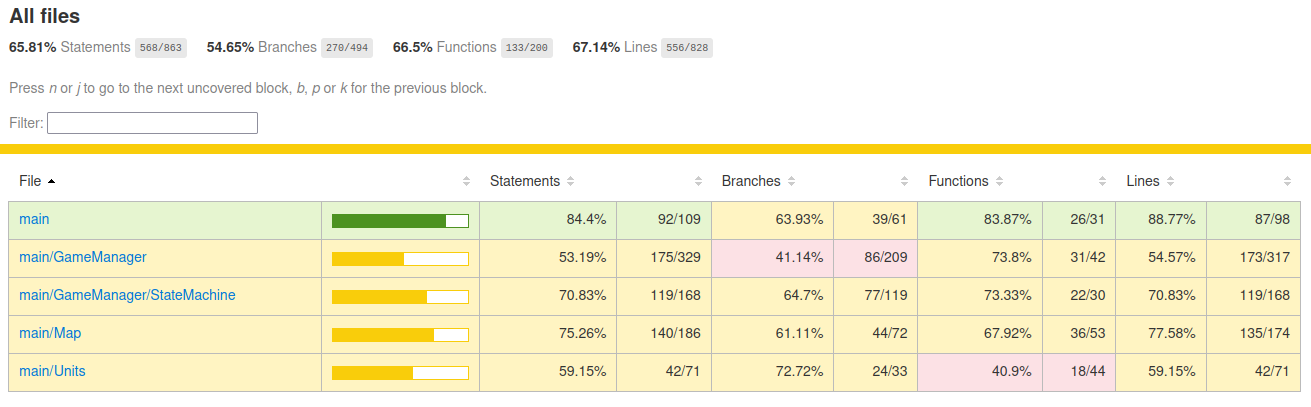
\includegraphics[scale=0.35]{data/couverture_test_1.png}
    \caption{Couverture générale du backend}
\end{figure}

On peut voir le pourcentage de couverture de chaque fichier. On peut aussi aller plus dans les détails et regarder ligne par ligne pour être sûr qu'absolument tout le code soit testé.

\begin{figure}[H]
    \centering
    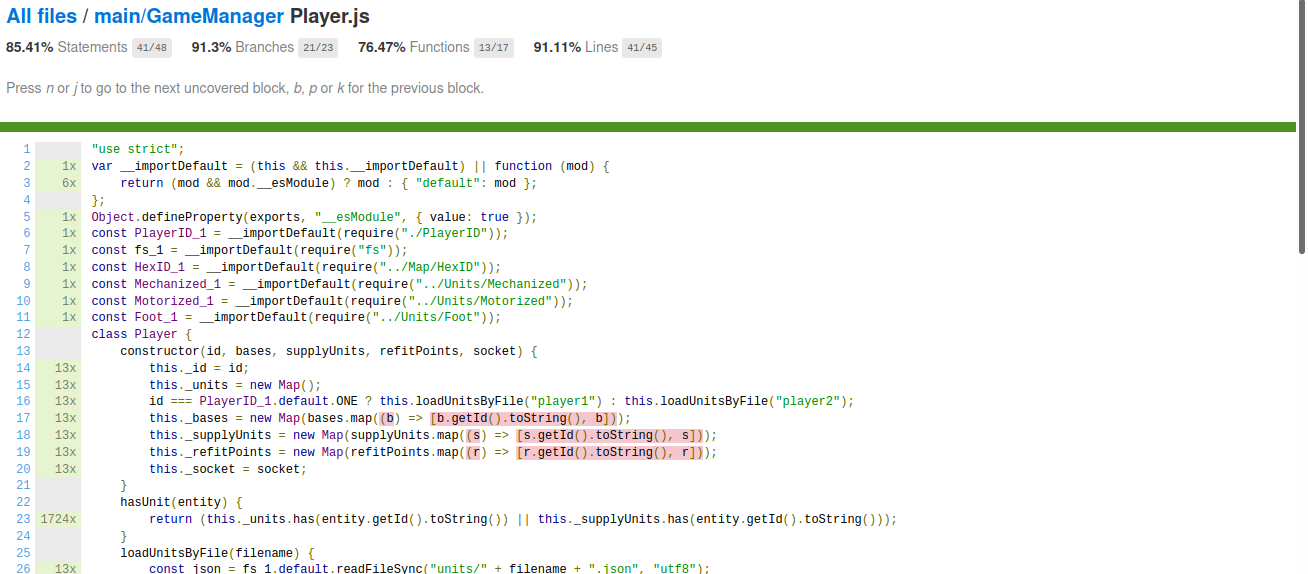
\includegraphics[scale=0.3]{data/couverture_test_2.png}
    \caption{Couverture d'un fichier}
\end{figure}

La couverture du code n'implique pas des tests de qualité. Après quelques recherches nous n'avons pas trouvé de ressource fiable, mais l'information qui ressortait le plus est qu'une bonne qualité de couverture dépasse les 80\%.
Nous nous sommes donc fixés d'au moins atteindre ce pourcentage. Un fichier dégrade notre {\tt coverage}, en effet nous ne testons pas main/GameManager/StateMachine/Command.ts car nous vérifions déjà dans le frontend que les commandes soumises aient les bons arguments.


\section{Conclusion}

Ce qu'il reste à faire :
\begin{itemize}
    \item Poser un cookie dans le client pour qu'il puisse reprendre une partie en cours s'il est déconnecté.
          Cela implique que la partie n'est pas directement détruite lorsqu'un joueur se déconnecte. Le serveur attendrait environs 3 minutes maximum avant de détruire la partie.
    \item Ajouter toutes les unités du jeu de base.
    \item Ajout de la mécanique {\tt overrun} qui permet l'attaque pendant la phase de mouvement.
    \item Ajout des phases: {\tt renforts}, {\tt allocation}, {\tt initiative}, {\tt aerial superiority}, {\tt supply attrition}, {\tt events}
          \begin{itemize}
              \item {\tt renforts}: Permet de ramener des unités détruites sur le terrain et les deux joueurs déterminent les unités disponibles comme renforts en cas d'attaque.
              \item {\tt allocation}: Permet d'activer les bases, construire des fortifications et entrainer les unités.
              \item {\tt initiative}: Lancer un dé permettant de déterminer quel joueur commence en premier.
              \item {\tt aerial superiority}: Permet de déployer ses unités aérienne puis de déterminer qui a l'avantage aérien.
                    La personne avec l'avantage peut faire des opérations aériennes.
              \item {\tt supply attrition}: Chaque joueur effectue un test de moral pour chaque unité qu'il possède afin de vérifier si son état devient {\tt disrupted} ou si elles deviennent isolées.
              \item {\tt events}: Permet de vérifier le status de tous les événements actifs. Chaque joueur déclare quels événements il veut provoquer.
          \end{itemize}
    \item Ajouter un temps de tour, c'est-à-dire que chaque joueur possède un certain temps pour jouer son tour. Actuellement si un jour ne fais rien, l'autre joueur doit attendre qu'il termine son tour.
    \item Ajouter tous les scénarios possibles du jeu de base.
\end{itemize}

L'un des problèmes majeurs rencontrés durant l'implémentation de ce projet est que les règles du jeu font 40 pages environs.
Cela qui nous a pris beaucoup de temps à comprendre et donc le début du développement du code a été retardé de quelques semaines.
De ce fait le projet n'est pas complétement fidèle aux règles du jeu de base.

Consigne : description de ce qu’il y aurait encore à faire, description des extensions possibles (et comment les réaliser).

\section{Bibliographie}


\bibliography{bibiography}

\subsection{Source images}

\printendnotes

\input{Annexe}



\end{document}
